\ifdefined\handoutmode
  \PassOptionsToClass{handout}{beamer}
\fi
\documentclass[aspectratio=169]{beamer}

\input{../../../../hh_bpa_forel-preamble} % this is ugly.

\title{FMTS mätteknik HT2026 -- Dag 1}
\author{Pererik Andreasson \\ Struan Gray }
\date{\today{}}

\begin{document}

%%% Title slide: different footer, large logo
{
% no page #, no logo on title page
\setbeamertemplate{footline}{}
\setbeamertemplate{logo}{\titlelogos}
\begin{frame}
\vfill
  \begin{block}
    \maketitle
  \end{block}
\end{frame}
}


% Lärarpresentation - foton
\mode<beamer>{
    \begin{frame}
    \begin{columns}
        \column{0.31\textwidth}    
            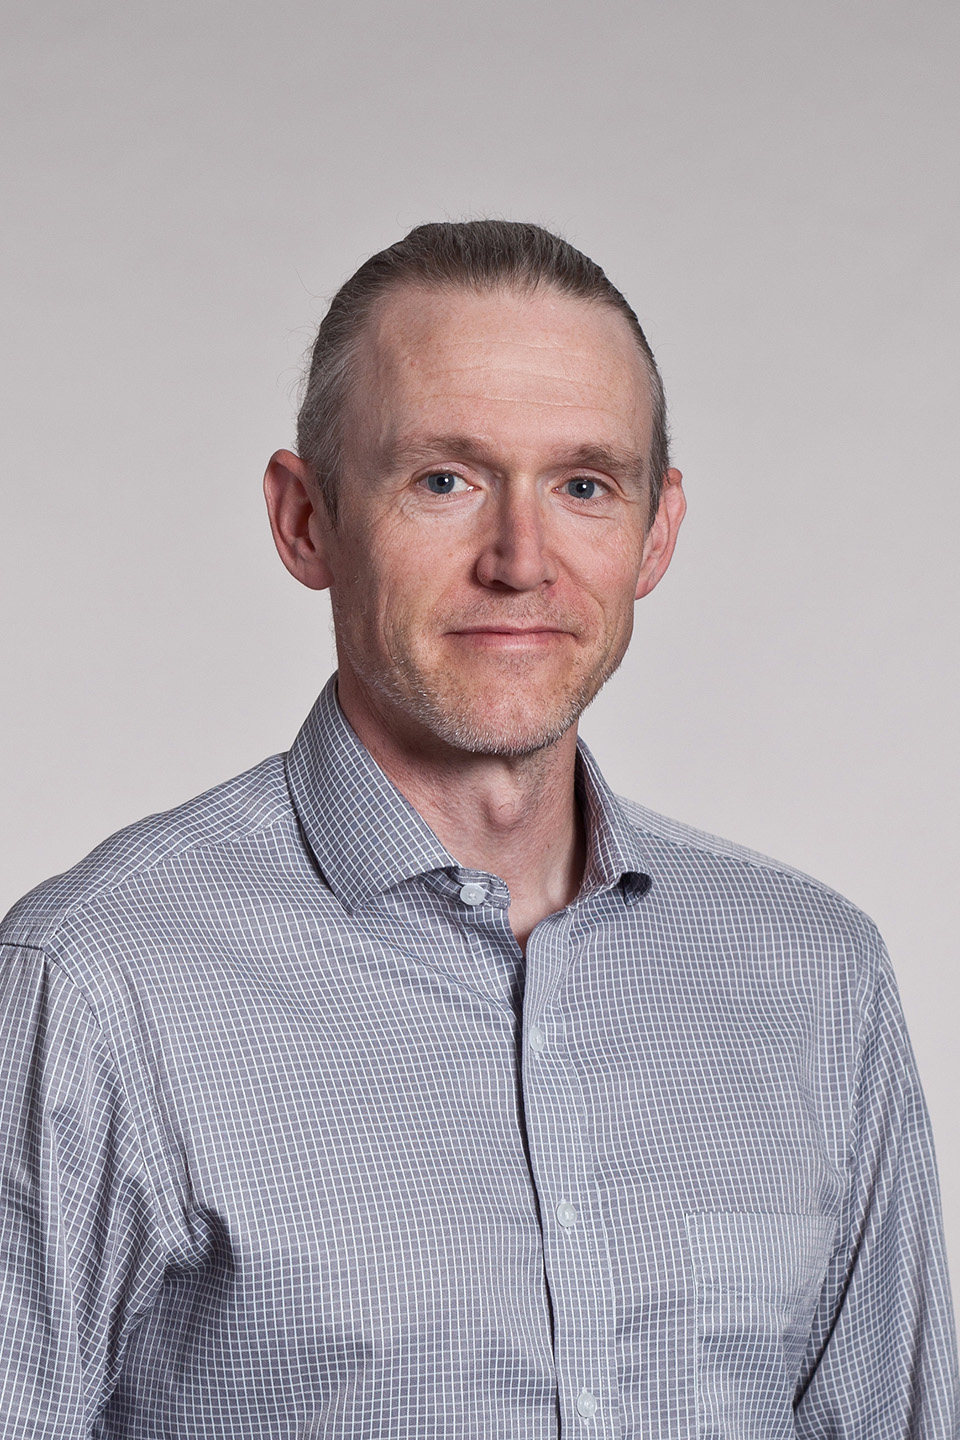
\includegraphics[width=\textwidth]{figures/pererik.jpg}\\
            Pererik -- Fysiker.
        \column{0.31\textwidth}    
            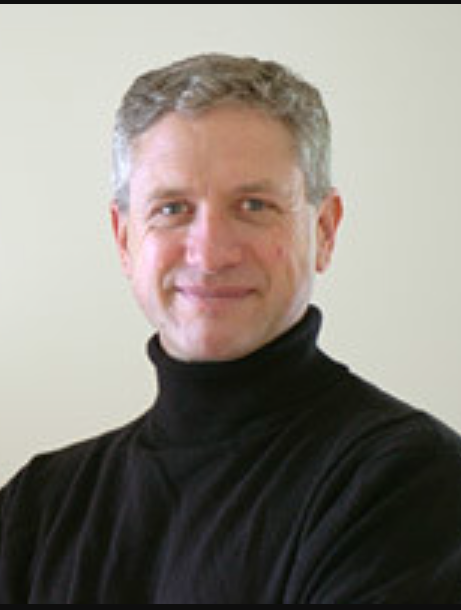
\includegraphics[width=\textwidth]{figures/struan.png}\\
            Struan -- Fysiker.
    \end{columns}
\end{frame}
} % mode

% Lärarpresentation - roligare foton
\mode<beamer>{
\begin{frame}
        \begin{columns}
        \column{0.31\textwidth}    
        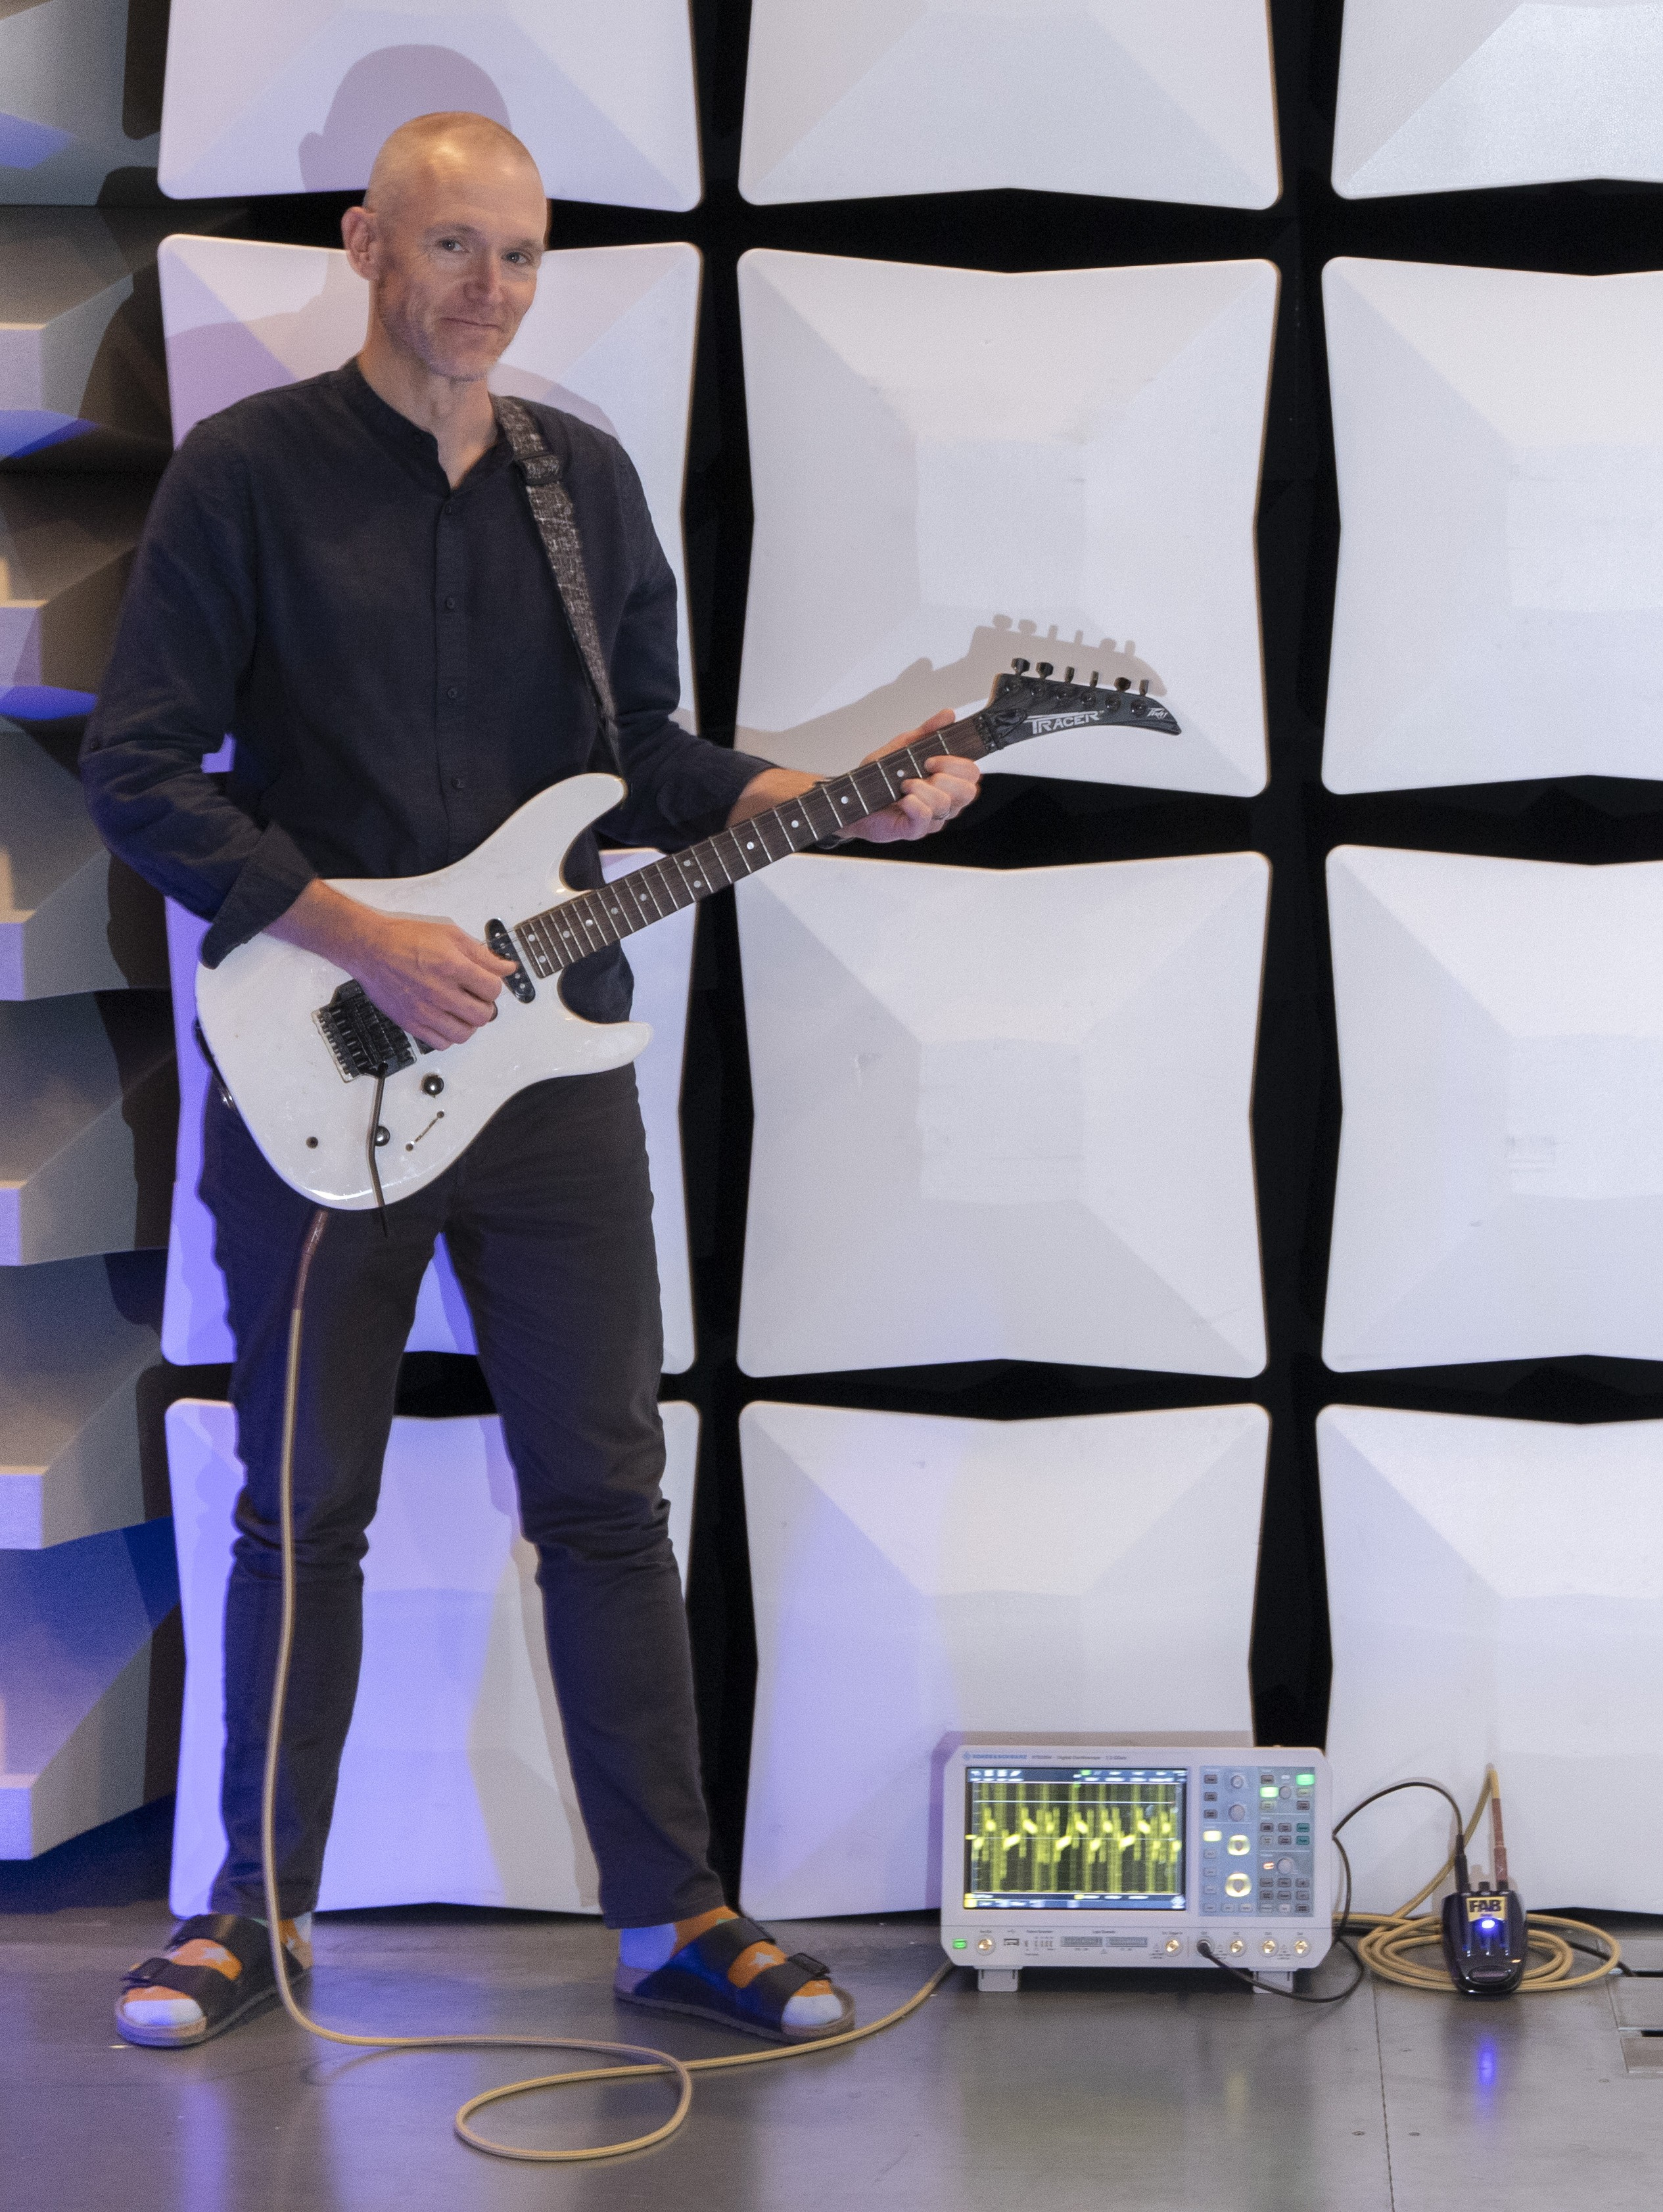
\includegraphics[width=\textwidth]{figures/pererik_gitarr.jpg}\\
        Pererik -- Fysiker.
        \column{0.31\textwidth}    
            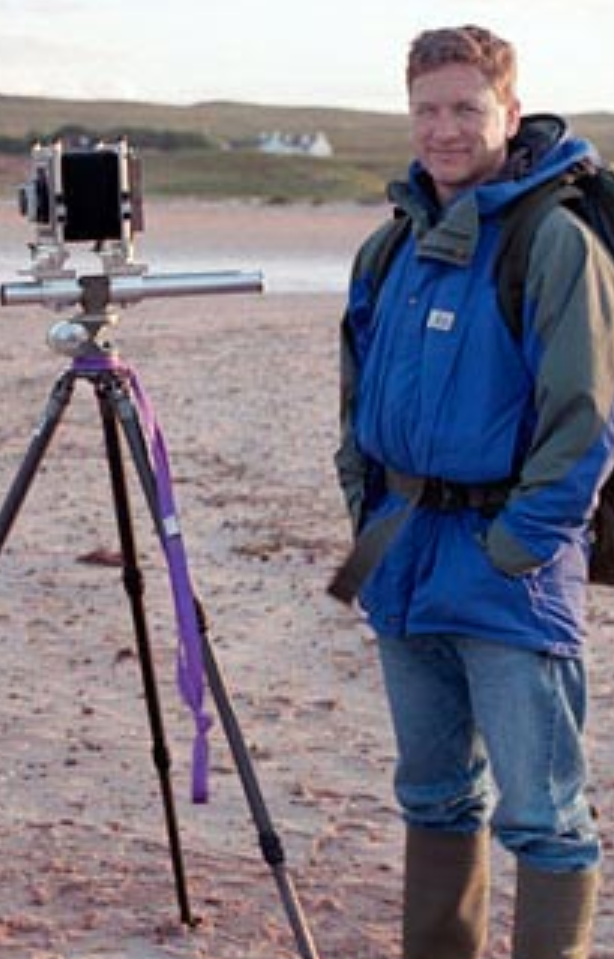
\includegraphics[width=\textwidth]{figures/struan_young.png}\\
            Struan -- Fysiker.
    \end{columns}
\end{frame}
} % mode

% kommando för att rita schemat (o)smidigt
\newcommand{\schedcell}[6]{%
    \path[
        draw,
        fill=#1
    ]
    (#2 |- #3) rectangle (#4 |- #5);

    \node[
        anchor=north west,
        align=left,
        text width={\dimexpr
            \ifx#2x0\TimeWidth\else\CellWidth\fi
            -6pt\relax}
    ]
    at ([xshift=3pt,yshift=-3pt]#2 |- #3)
    {#6};
}

% schemabilden (kommandot utanför annars kaputt)
\begin{frame}{Schema}

% =================================================
% PARAMETERS
% =================================================
\newcommand{\ScheduleFontSize}{10.5} % font size in pt
\newcommand{\ScheduleShift}{0mm}     % shift entire schedule to the left

\newcommand{\CellWidth}{2.60cm}      % width of ordinary cells
\newcommand{\CellHeight}{1.25cm}     % height of all rows
\newcommand{\TimeWidth}{2.25cm}      % width of time column

\pgfmathsetmacro{\ScheduleBaseline}{1.20*\ScheduleFontSize}

\centering
\makebox[\textwidth][c]{%
\hspace*{-\ScheduleShift}%

\begin{tikzpicture}[
    font=\fontsize{\ScheduleFontSize pt}
                   {\ScheduleBaseline pt}\selectfont,
    line width=0.5pt,
    every node/.style={inner sep=3pt}
]

% =================================================
% COLORS
% =================================================
\definecolor{timecol}{RGB}{240,240,240}
\definecolor{pcol}{RGB}{220,235,250}
\definecolor{ecol}{RGB}{250,232,210}
\definecolor{pecol}{RGB}{228,222,245}
\definecolor{introcol}{RGB}{225,240,225}


% =================================================
% COLUMN AND ROW POSITIONS
%
% Change ONLY \CellWidth, \CellHeight and
% \TimeWidth above to resize the schedule.
% =================================================

\coordinate (x0) at (0,0);
\coordinate (x1) at ([xshift=\TimeWidth]x0);
\coordinate (x2) at ([xshift=\CellWidth]x1);
\coordinate (x3) at ([xshift=\CellWidth]x2);
\coordinate (x4) at ([xshift=\CellWidth]x3);
\coordinate (x5) at ([xshift=\CellWidth]x4);
\coordinate (x6) at ([xshift=\CellWidth]x5);

\coordinate (y0) at (0,0);
\coordinate (y1) at ([yshift=-\CellHeight]y0);
\coordinate (y2) at ([yshift=-\CellHeight]y1);
\coordinate (y3) at ([yshift=-\CellHeight]y2);
\coordinate (y4) at ([yshift=-\CellHeight]y3);


% =================================================
% HELPER COMMAND
%
% #1 = color
% #2 = upper-left x coordinate
% #3 = upper y coordinate
% #4 = lower-right x coordinate
% #5 = lower y coordinate
% #6 = contents
% =================================================

% =================================================
% 08.00--10.00
% =================================================

\schedcell{timecol}{x0}{y0}{x1}{y1}{08.00--10.00}

\schedcell{white}{x1}{y0}{x2}{y1}{}

\schedcell{pcol}{x2}{y0}{x3}{y1}{%
    \textbf{Multimeter}\\
    S
}

\schedcell{pecol}{x3}{y0}{x4}{y1}{%
    \textbf{Oscilloskop}\\
    P
}

\schedcell{pecol}{x4}{y0}{x5}{y1}{%
    \textbf{Oscilloskop}\\
    P
}

\schedcell{introcol}{x5}{y0}{x6}{y1}{%
    \textbf{Buffert}\\
    S
}


% =================================================
% 10.00--12.00
% =================================================

\schedcell{timecol}{x0}{y1}{x1}{y2}{10.00--12.00}

\schedcell{white}{x1}{y1}{x2}{y2}{}

\schedcell{pcol}{x2}{y1}{x3}{y2}{%
    \textbf{Multimeter}\\
    S
}

\schedcell{pecol}{x3}{y1}{x4}{y2}{%
    \textbf{Oscilloskop}\\
    P
}

\schedcell{pecol}{x4}{y1}{x5}{y2}{%
    \textbf{Oscilloskop}\\
    P
}

\schedcell{introcol}{x5}{y1}{x6}{y2}{%
    \textbf{Avslutning}\\[2mm]
    P + S
}


% =================================================
% 13.00--15.00
% =================================================

\schedcell{timecol}{x0}{y2}{x1}{y3}{13.00--15.00}

\schedcell{pcol}{x1}{y2}{x2}{y3}{%
    \textbf{Intro P + S}\\
    ``Statistik''
}

\schedcell{pcol}{x2}{y2}{x3}{y3}{%
    \textbf{Multimeter}\\
    P
}

\schedcell{pecol}{x3}{y2}{x4}{y3}{%
    \textbf{Oscilloskop}\\
    P
}

\schedcell{ecol}{x4}{y2}{x5}{y3}{%
    \textbf{Effektmätare}\\
    P
}


% =================================================
% 15.00--17.00
% =================================================

\schedcell{timecol}{x0}{y3}{x1}{y4}{15.00--17.00}

\schedcell{pcol}{x1}{y3}{x2}{y4}{%
    \textbf{Ellära S}
    Multimeter
}

\schedcell{pcol}{x2}{y3}{x3}{y4}{%
    \textbf{Multimeter}\\
    S
}

\schedcell{pecol}{x3}{y3}{x4}{y4}{%
    \textbf{Oscilloskop}\\
    P
}

\schedcell{ecol}{x4}{y3}{x5}{y4}{%
    \textbf{Effektmätare}\\
    P
}

\end{tikzpicture}%
\hspace*{\ScheduleShift}%
}

\end{frame}


\mode<beamer>{
\begin{frame}
    \frametitle{}
    {\Huge Nyckelkort (sal låst) och telefonkedja (snabba ändringar).}    
\end{frame}
} % mode

% motivering för mätteknik
\mode<beamer>{
\descriptionslide{figures/voltmeter_in_action.jpg}{1}
    {Varför behöver vi förstå mätteknik?}{}
} % mode

\descriptionslide{figures/anteckna.jpg}{1}
    {Läromedel och anteckningar}{}

\handoutnoteslide{Dessa tomma rutor är till för anteckningar.}


\begin{frame}
    \frametitle{Lärandemål}
    {\Huge
    \begin{enumerate}
        \item<2-> Ensam mätning inget värt.
        \item<3-> Okalibrerat mätinstrument inget värt.
        \item<4-> Elektriska mätningar \emph{påverkar} mätobjektet $\rightarrow$ behöver \emph{tolkas}.
    \end{enumerate}
    }
\end{frame}

\handoutnoteslide

\mode<beamer>{
\frame{
    \begin{columns}
        \column{0.3\textwidth}    
            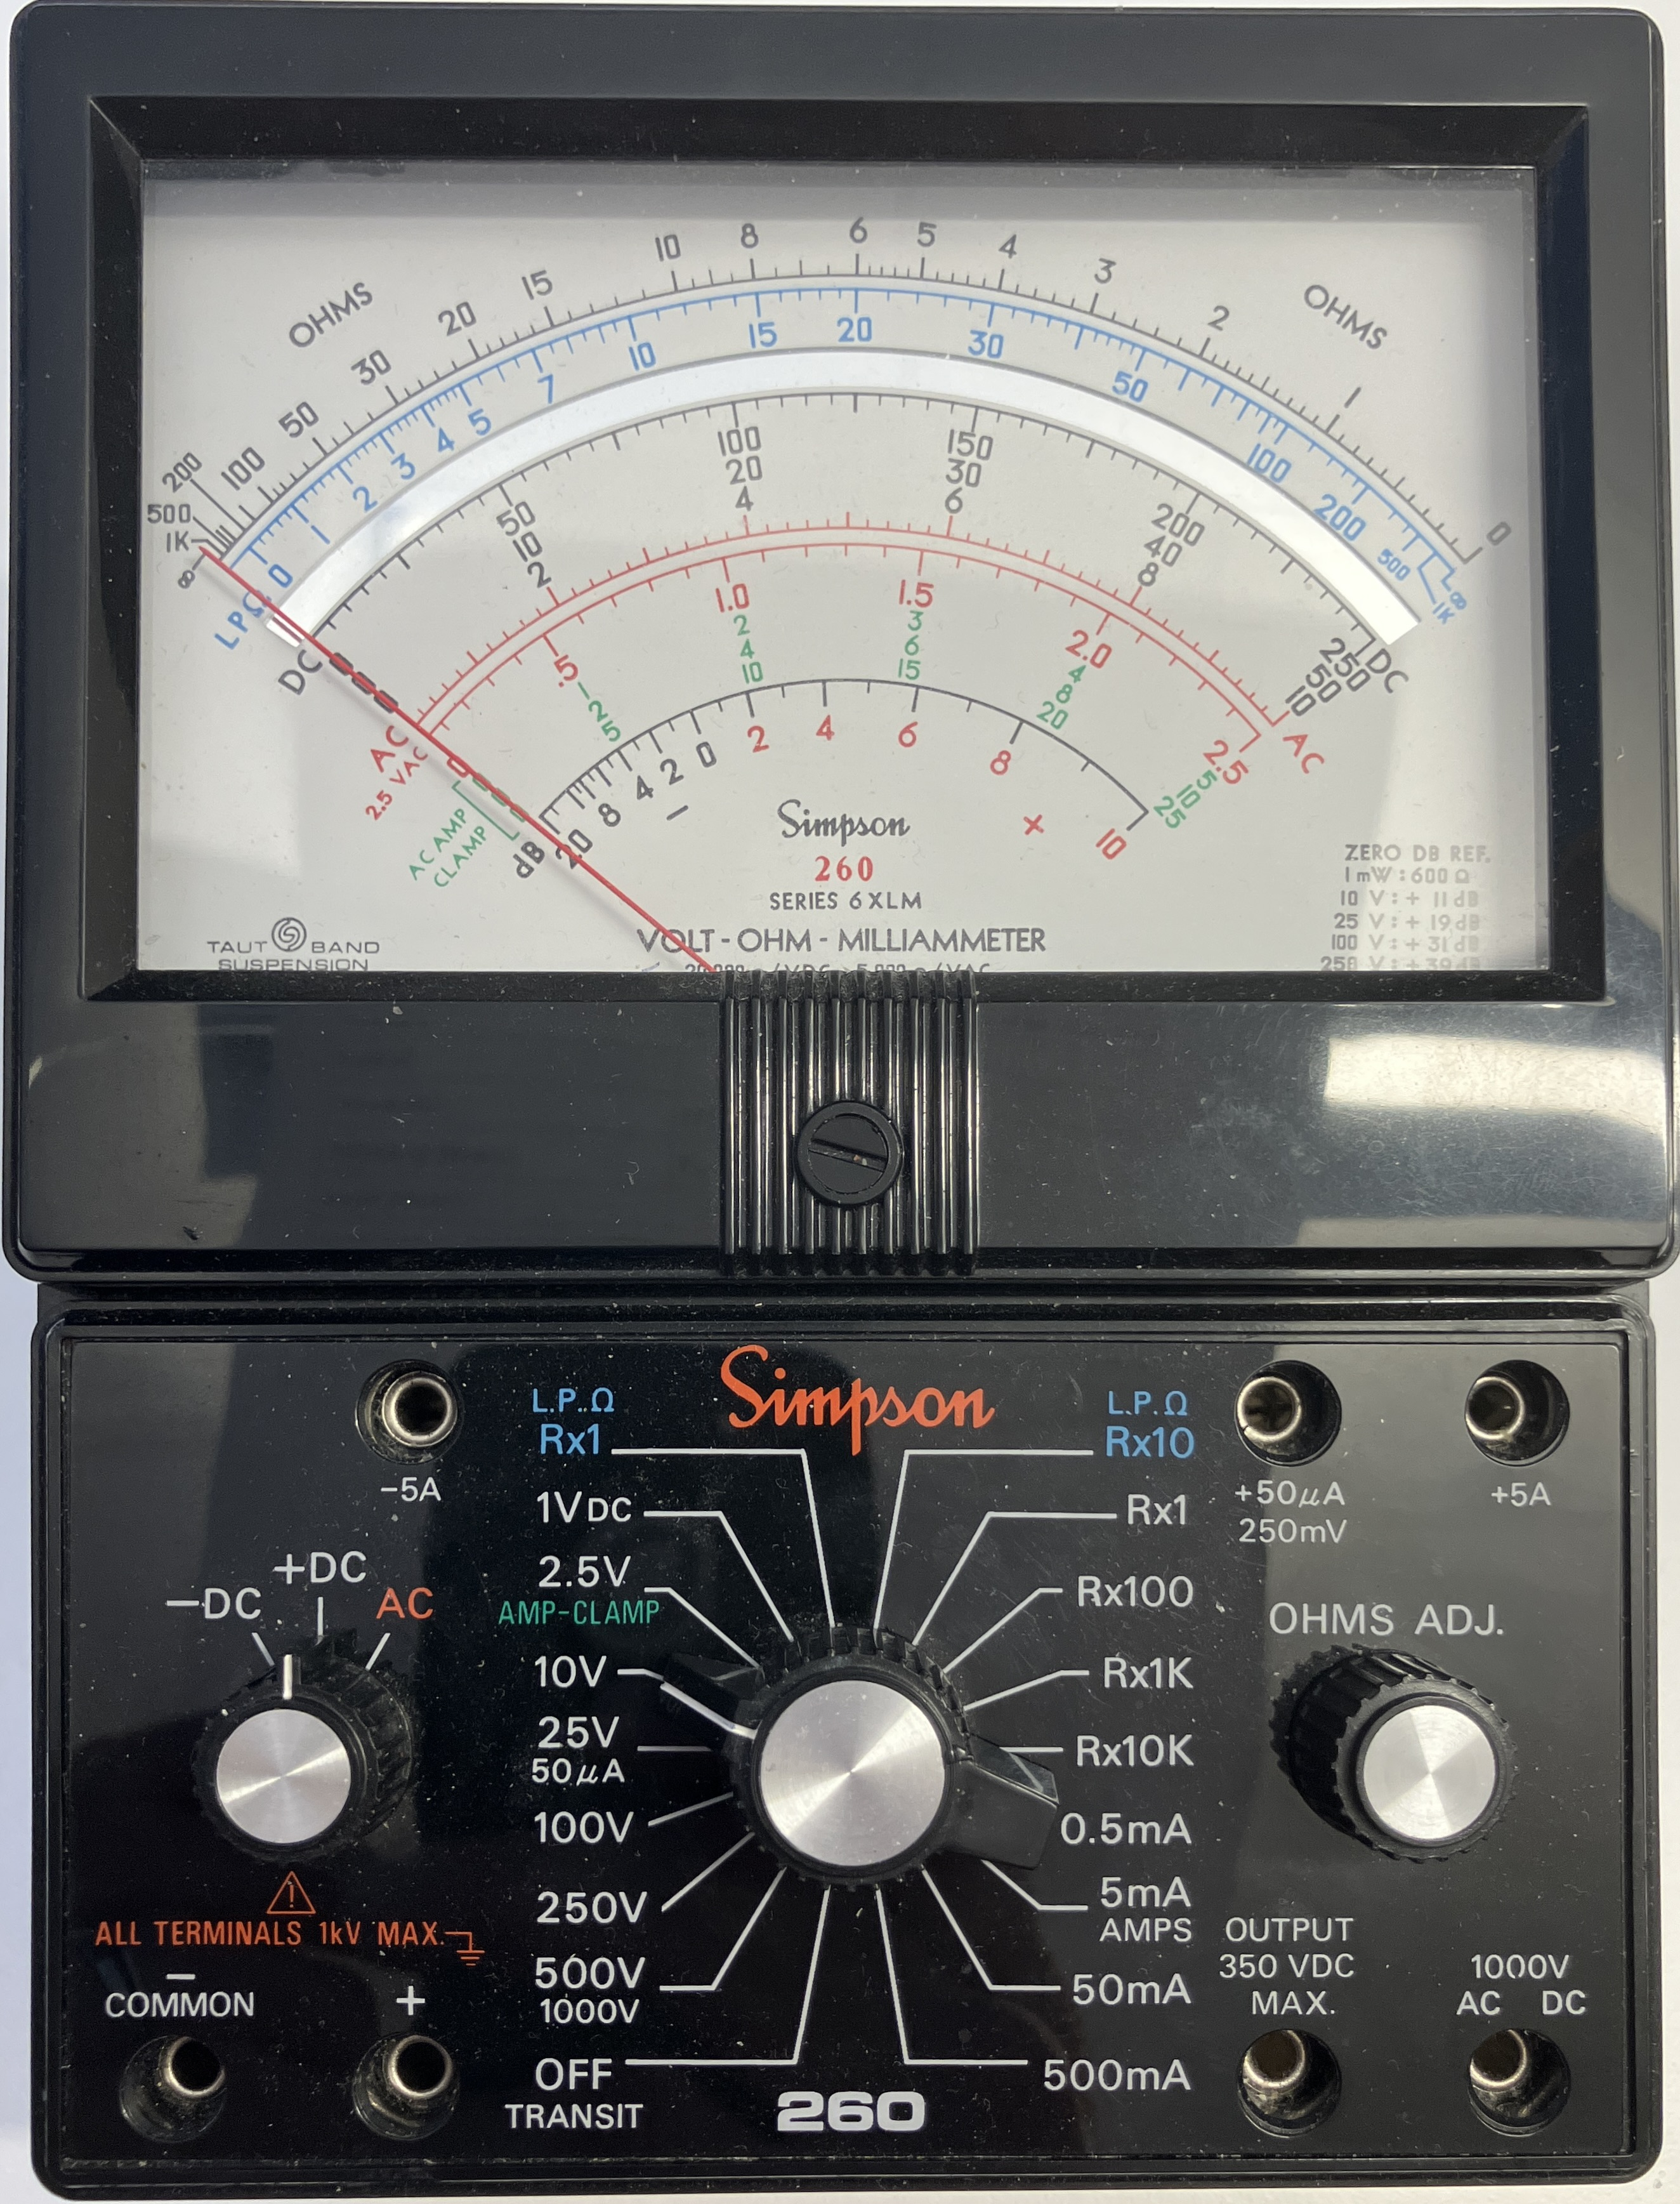
\includegraphics[height=0.45\textheight]{figures/multimeter_analog.jpg}
        \column{0.3\textwidth}<2->
            \centering
            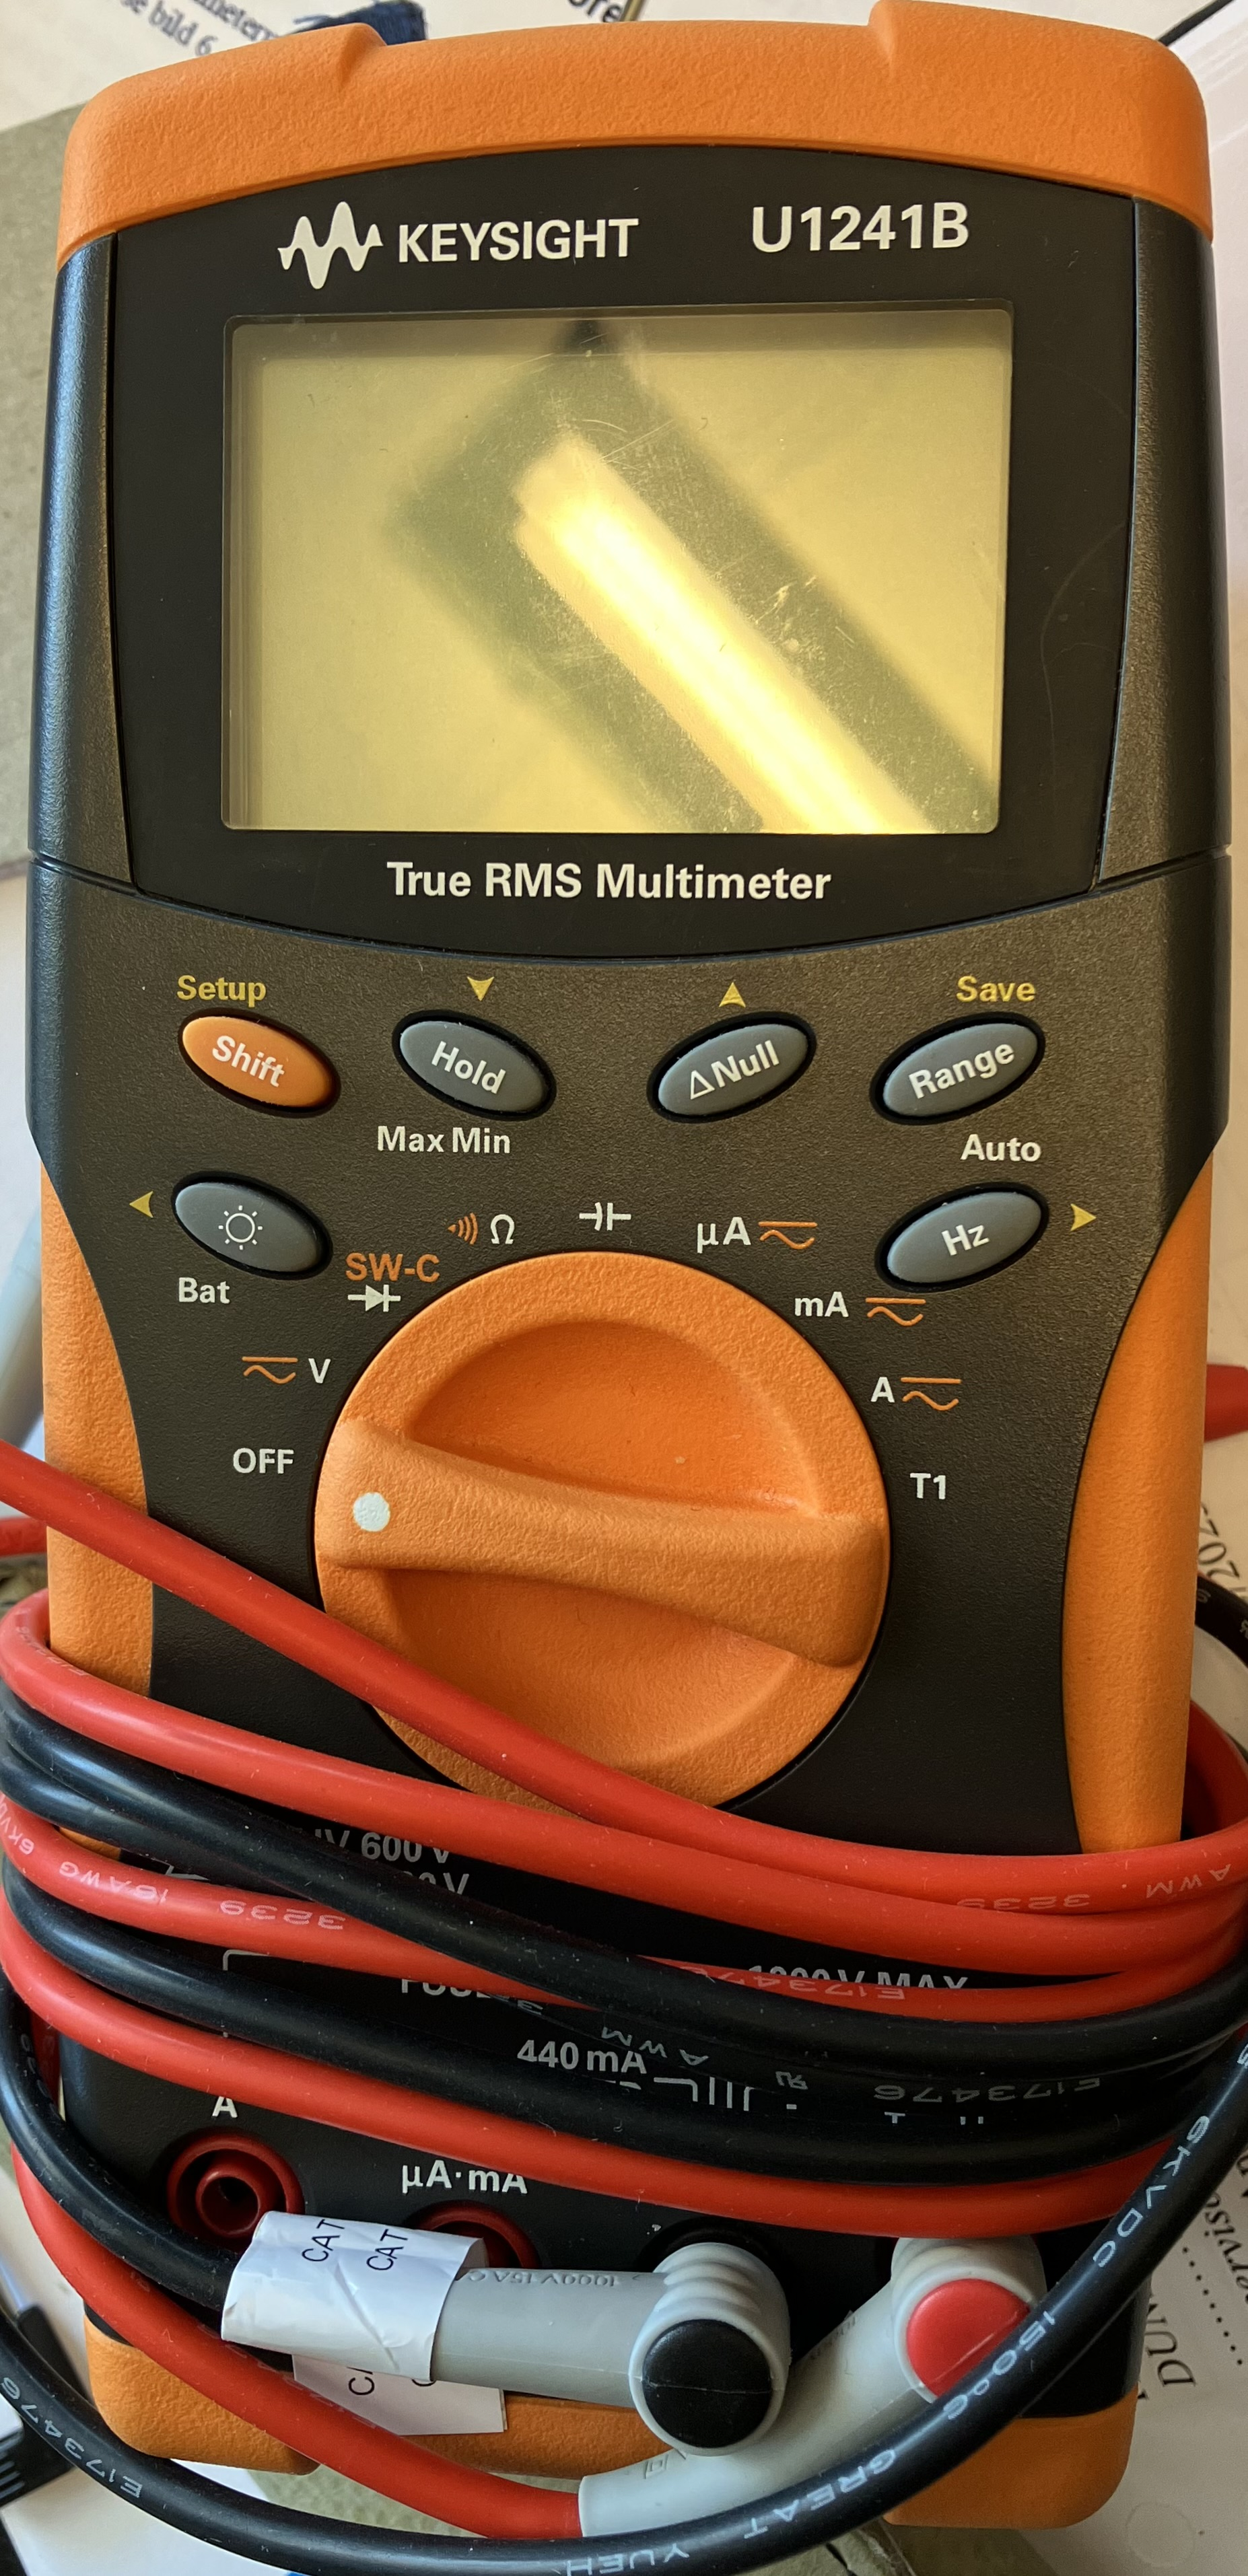
\includegraphics[height=0.45\textheight]{figures/dmm.jpg}
        \column{0.3\textwidth}<4->    
            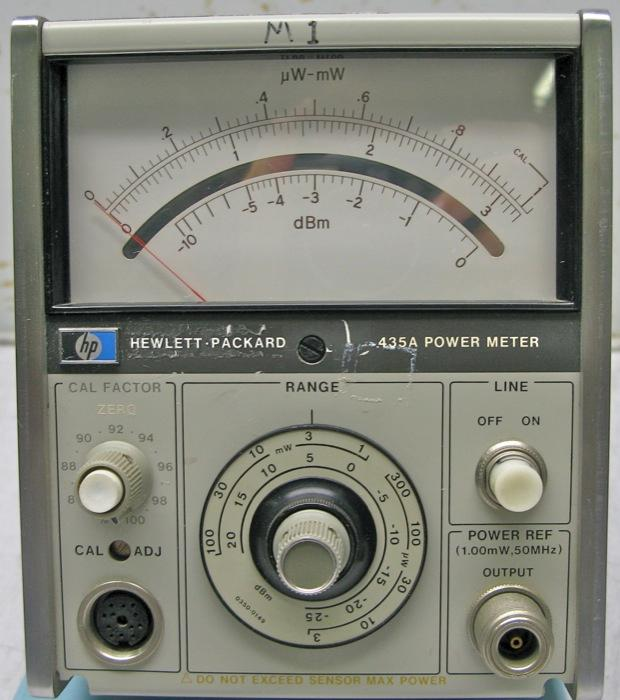
\includegraphics[height=0.45\textheight]{figures/powermeter.jpg}
    \end{columns}
    \vspace{5mm}
    \begin{columns}
        \column{0.5\textwidth}<3->    
            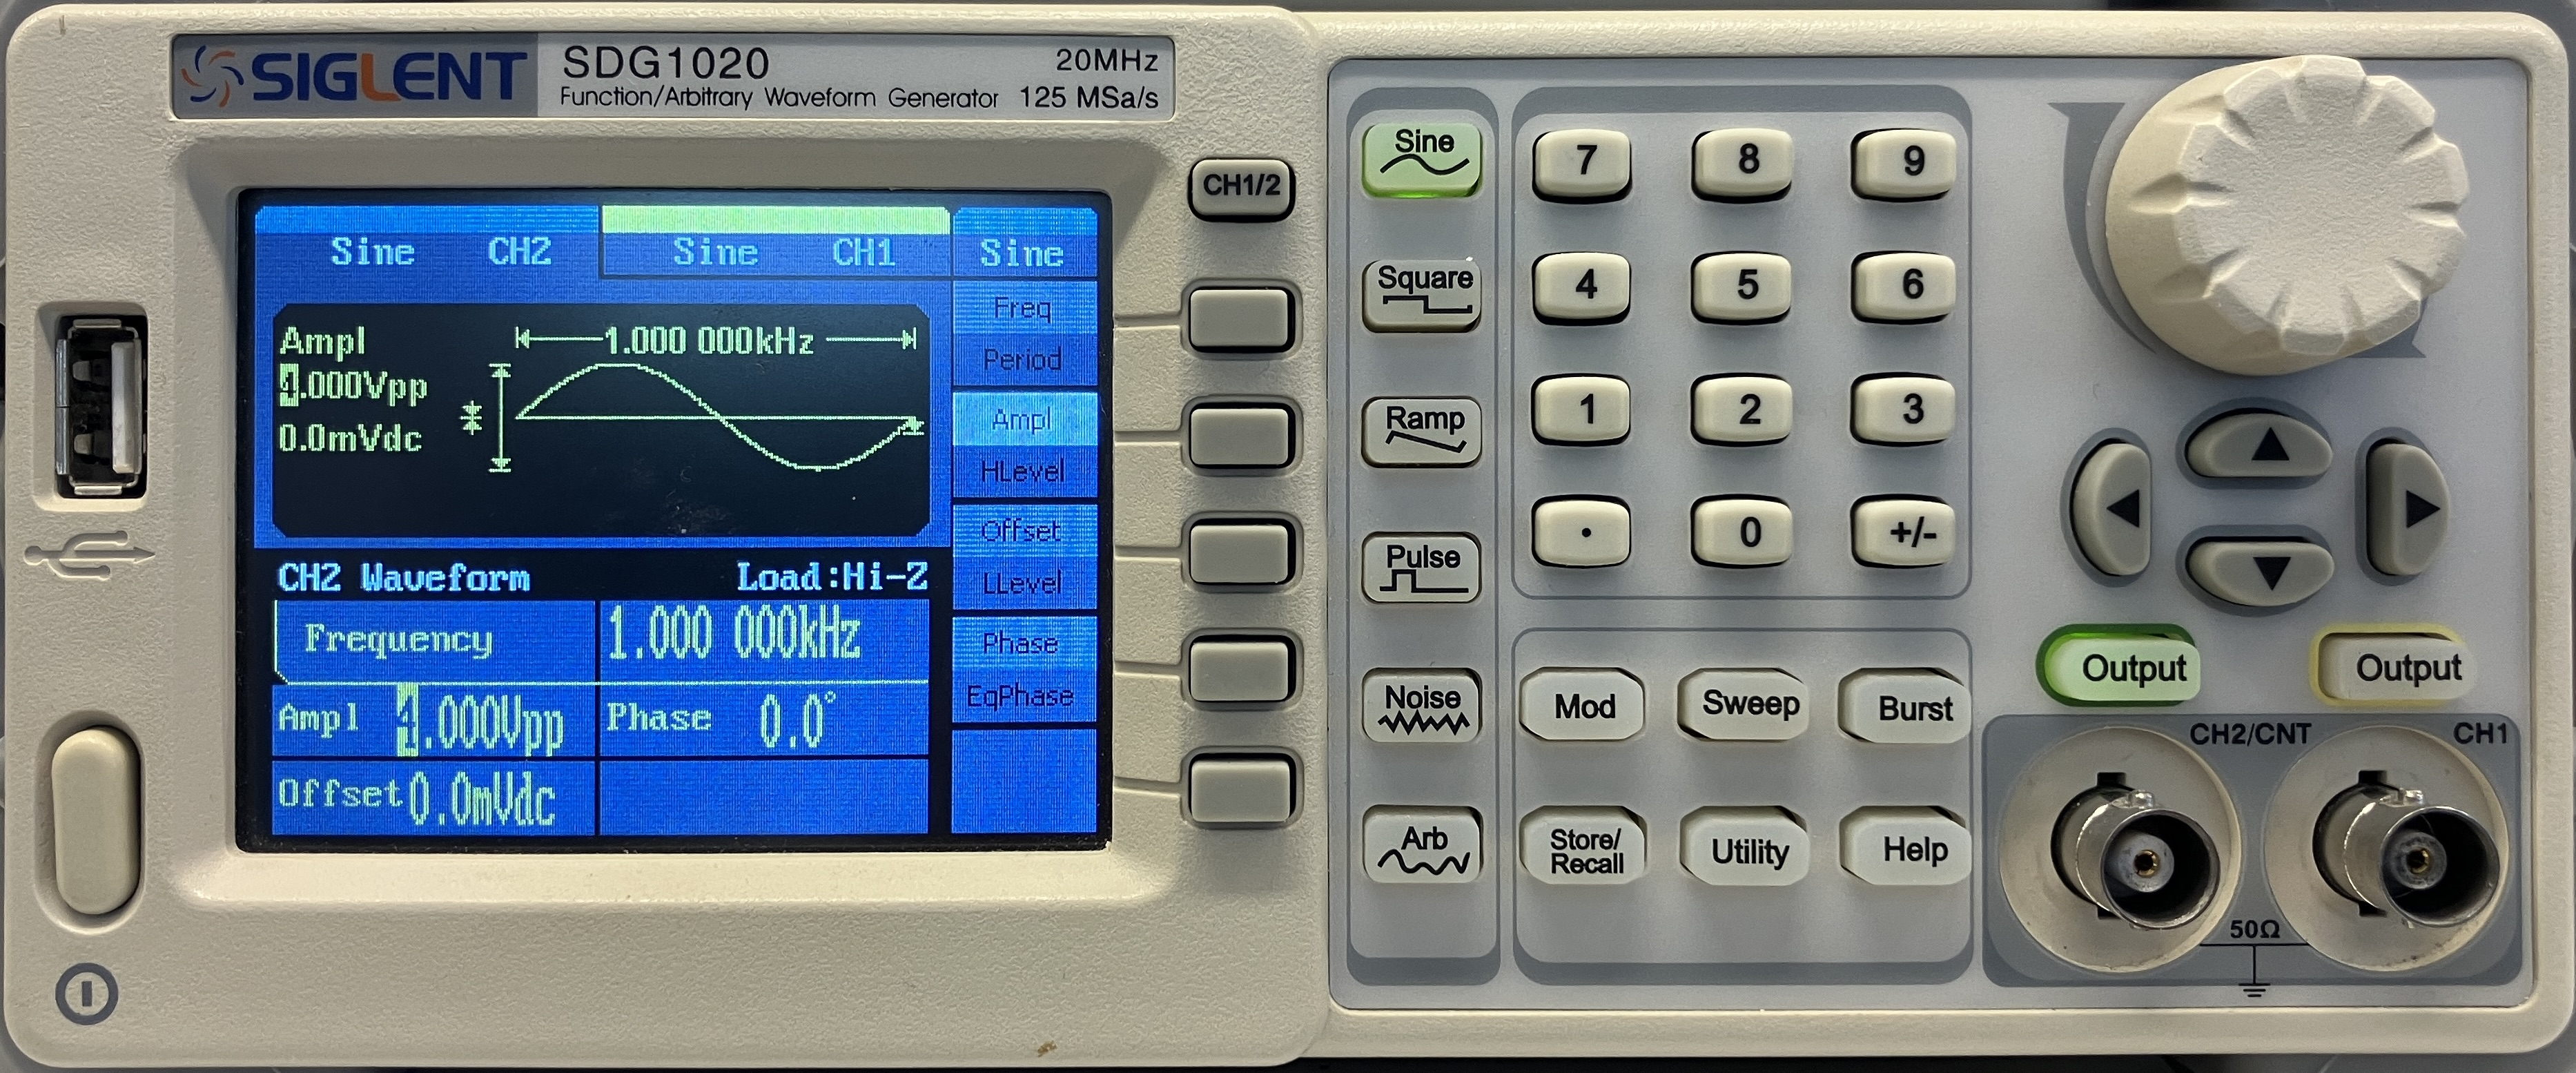
\includegraphics[width=\textwidth]{figures/signalgenerator.jpg}
        \column{0.5\textwidth}<3->    
            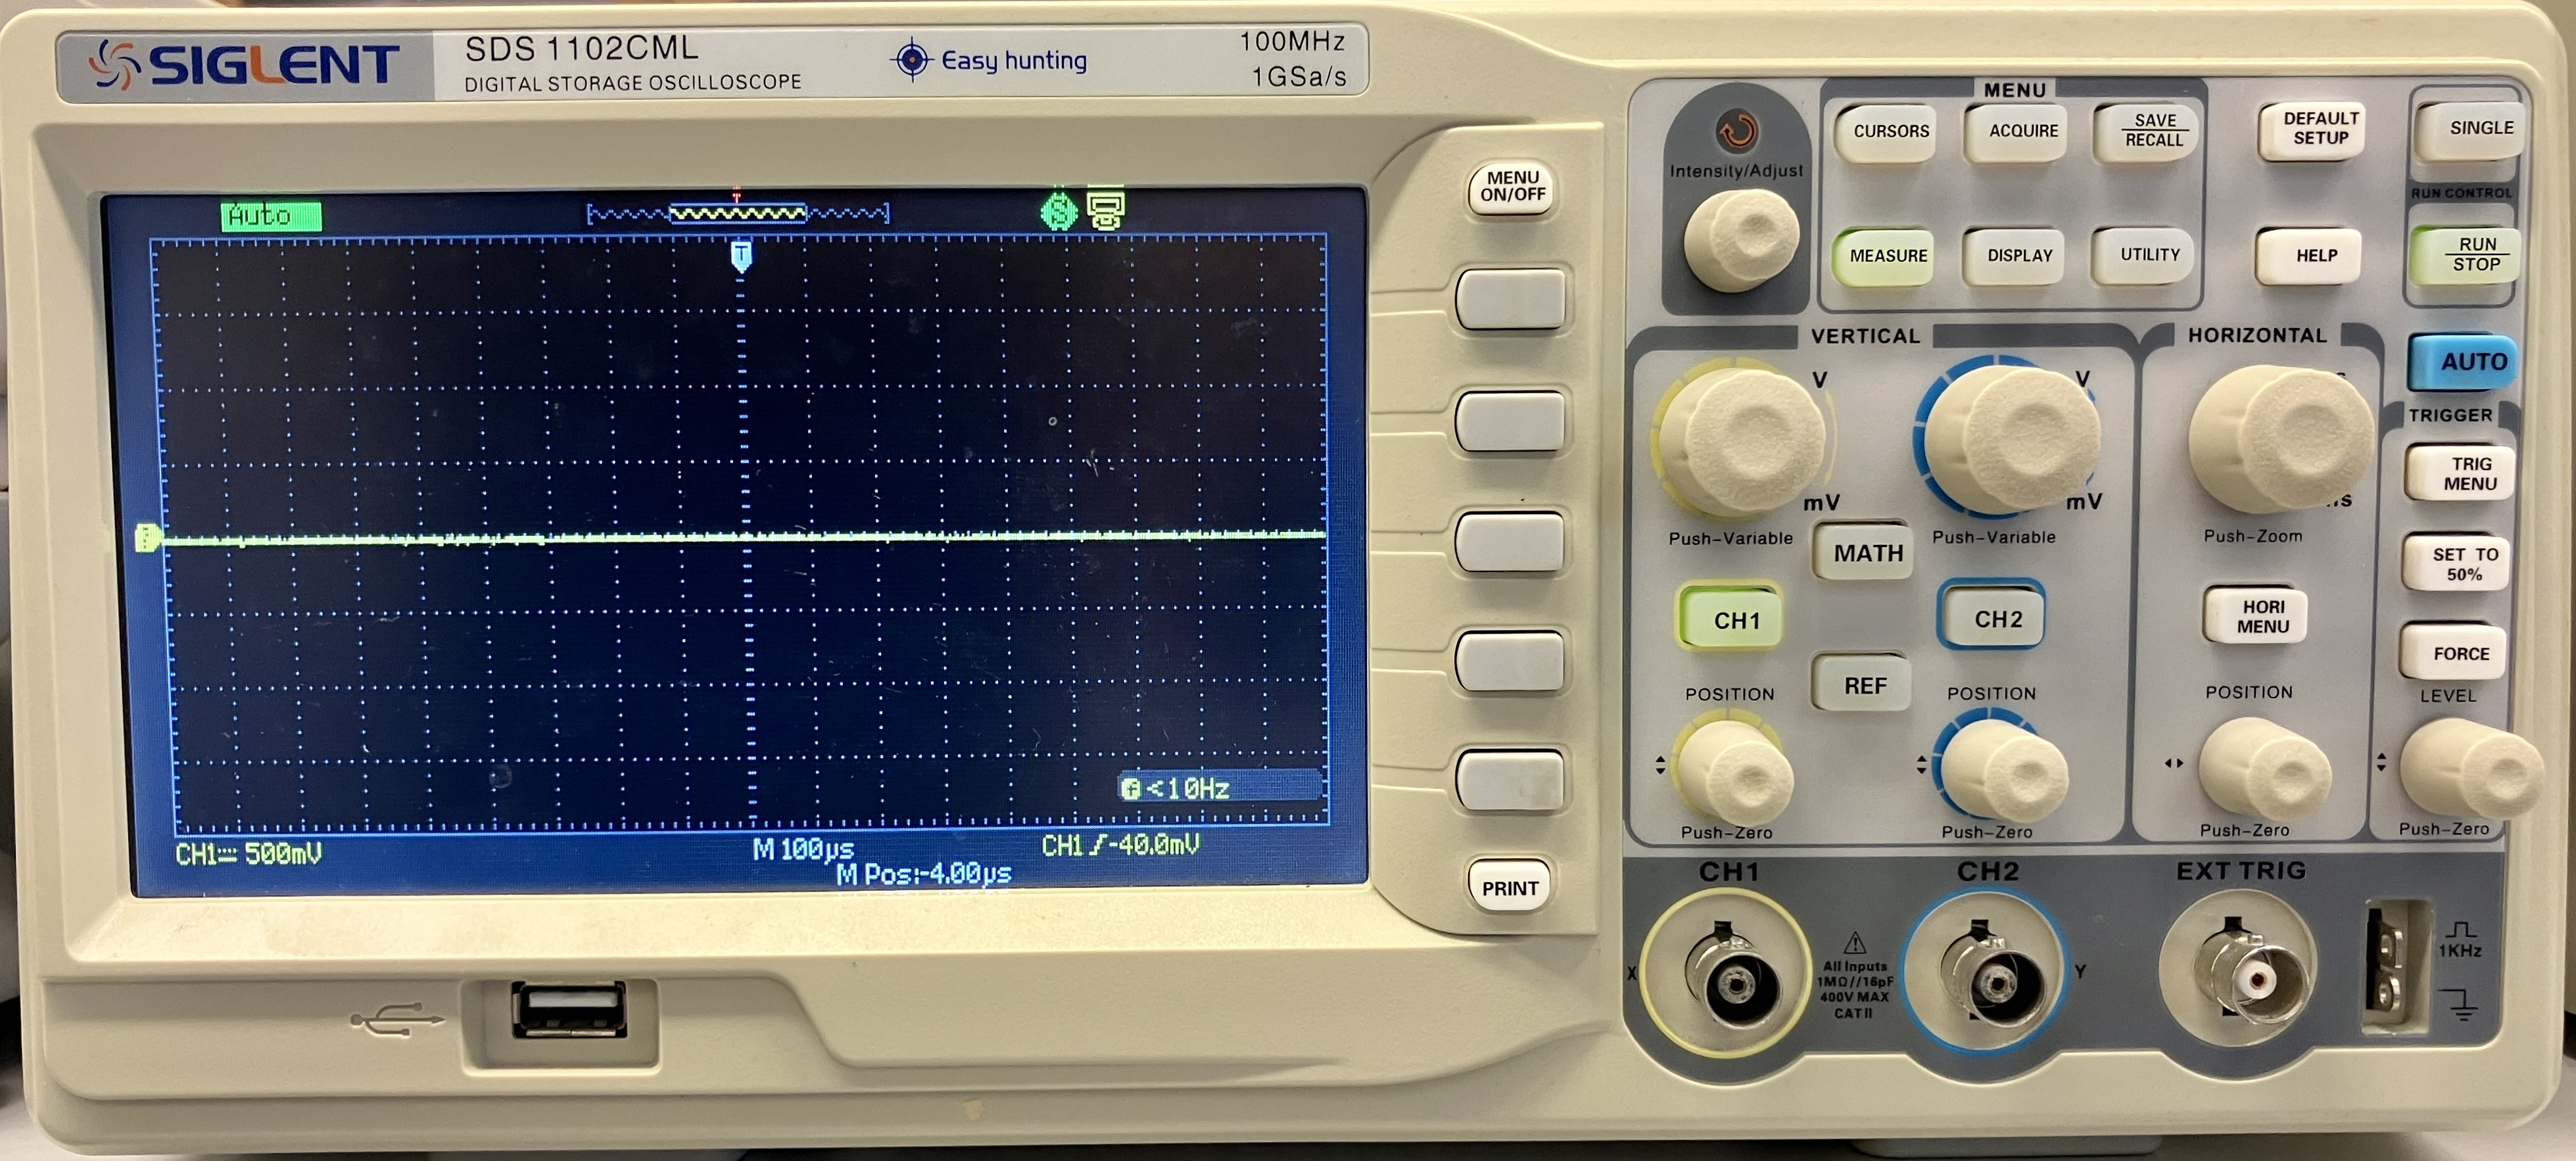
\includegraphics[width=\textwidth]{figures/oscilloskop.jpg}
    \end{columns}
    }
} % mode


\frame{
    \frametitle{Dagens plan}
    {\huge
        \begin{itemize}
            \item Mäta längden på en briotågbanerälsbit och låtsas förstå statistik.
            \item Introlabba lite.
            \item Repetera ellära.
            \item Mäta med multimeter.
        \end{itemize}
    }
    }   

% section här skall vara kvar - annars fel på sidor nedan.
    \sectionslide{Oberoende mätningar}

\frame{
    \frametitle{Enheter och storheter}
    {\Large 
    \begin{columns}
        \column{0.6\textwidth}
    Storhet -- något du kan mäta\\\vspace{2mm}
    Enhet -- måttet på en storhet\\\vspace{2mm}        
        \column{0.3\textwidth}
            \begin{align*}
            	\underbrace{U}_\text{Storhet}=
	            \underbrace{234}_\text{Mätetal}
	            \underbrace{\unit{\V}}_\text{Enhet}
            \end{align*}
    \end{columns}
    \vspace{5mm}
\onslide<2-> De sju SI-enheterna (dödssynderna)
\begin{columns}
\begin{column}{0.5\textwidth}
    \begin{itemize}
        \item<3-> Längd -- (m)
    	\item<3-> Massa -- (kg)
    	\item<3-> Tid -- (s)
    	\item<3-> Ström -- (A)
    	\item<3-> Temperatur -- (K)
     \end{itemize}
\end{column}
\begin{column}{0.5\textwidth}
    \begin{itemize}

    	\item<4-> Ljusstyrka -- (cd)
    	\item<4-> Antal molekyler -- (mol)
    \end{itemize}
\vspace{5mm}
\onslide<5->{Volt -- \unit{\kg\m\squared\per\s\cubed\per\A}}

\end{column}
\end{columns}
    } % fontsize
    } % frame end 

\handoutnoteslide

\frame{
    \frametitle{Potensform och prefix}
    \begin{columns}
        \column{0.5\textwidth}
            \begin{align*}
                100 &= 1 \times 10 \times 10 \\
                &= 1 \times 10^2\\
                \onslide<2->{10000 &= 1 \times 10 \times 10 \times 10 \times 10 \\
                &= 1 \times 10^4\\}
                &\\
                \onslide<3->{0.001 &= \frac{1}{10 \times 10 \times 10}\\
                &= \frac{1}{10^3}
                = 1 \times 10^{-3}\\}
                &\\
                \onslide<4->{1500 &= 1.5 \times 10^{3}\\
                0.015&= 1.5 \times 10^{-2}} \onslide<5->{= \num{15e-3}}
            \end{align*}
        \column{0.5\textwidth}
            \onslide<6->{
            
            \begin{table}
                \centering
            \resizebox{0.9\textwidth}{!}{
                \begin{tabular}{lll}
                    T & tera & $10^{12}$\\
                    G & giga & $10^9$\\
                    M & mega & $10^6$\\
                    k & kilo & $10^3$\\
                    - & - & $10^0$\\
                    m & milli & $10^{-3}$\\
                    $\mu$ & micro & $10^{-6}$\\
                    n & nano & $10^{-9}$\\
                    p & pico & $10^{-12}$
                \end{tabular}
            } % resizebox
            \end{table}
            } % onslide
    \end{columns}
}

\handoutnoteslide

\begin{frame}
    \frametitle{Mätningar och data}
    \begin{columns}
        \column{0.2\textwidth}<1->
  
\includegraphics[width=\textwidth]{figures/legofigur.png}
        \column{0.8\textwidth}<2->
	\begin{tikzpicture}
		\begin{axis}[
			xlabel={Mätning (nummer)},
			ylabel={Figurhöjd (\unit{\cm})},
			xmin=-2,
			xmax=201,
			ymin=2.7,
			ymax=5.3,
			width=90mm,
			every axis y label/.style={
            at={(ticklabel cs:0.5)},rotate=90,anchor=near ticklabel,
        },
			]
			\addplot [only marks] table [col sep=comma] {data/legofigurdata_20240811.csv} ;
		\end{axis}
	\end{tikzpicture}
    \end{columns}
\end{frame}


\handoutnoteslide


\begin{frame}
    \frametitle{Mätningar och data}
    \begin{columns}
        \column{0.2\textwidth}
  
\includegraphics[width=\textwidth]{figures/legofigur.png}
        \column{0.8\textwidth}
    \begin{tikzpicture}
		\begin{axis}[
			xlabel={Figurhöjd (\unit{\cm})},
			ylabel={Antal mätningar},
			width=90mm,
			every axis y label/.style={
            at={(ticklabel cs:0.5)},rotate=90,anchor=near ticklabel,},
			]
			\addplot [hist={bins=10}] table [col sep=comma] {data/legofigurdata_20240811.csv} ;
		\end{axis}
	\end{tikzpicture}
    \end{columns}
\end{frame}

\handoutnoteslide

% histogram, accuracy, precision
\begin{frame}[fragile]
    \frametitle{M\"atfel -- noggrannhet}
    \begin{columns}
    \column{0.6\textwidth}
    	\resizebox{\textwidth}{!}{
    	\begin{tikzpicture}
		\begin{axis}[
			xlabel={Mätvärde (t.ex. figurhöjd)},
			ylabel={Sannolikhetsdensitet},
            axis lines = left,
			width=80mm,
            xmax = 8,
            xmin = -4,
            ymax = 150,
            xtick=\empty,
            ytick=\empty,
			every axis y label/.style={
            at={(ticklabel cs:0.5)},rotate=90,anchor=near ticklabel,},
			every axis x label/.style={
            at={(ticklabel cs:0.5)},anchor=near ticklabel,},
			]
			\addplot [hist={bins=10}] table [col sep=comma] {../dag01/data/legofigurdata_20240811.csv} ;
            	
            	\draw[ultra thick, red, visible on=<2->] (axis cs:3.75, 0) -- (3.75, 150) node[below, black] {Uppmätt} ;             	
            	
            	\draw[<->, ultra thick, dashed, visible on=<3->] (axis cs:2,25) -- (5.5,25) node[midway, above] {Precision} ;
            	
            	\draw[ultra thick, red, visible on=<4->] (axis cs:-1.1, 0) -- (-1.1, 150)  node[below, black] {''Sant''};

            	\draw[<->, ultra thick, dashed, visible on=<5->] (axis cs:-1.1,100) -- (3.75,100) node[midway, above] {Noggrannhet} ;
		\end{axis}
	\end{tikzpicture}
	} % resizebox
    \column{0.4\textwidth}
		{\LARGE
    \begin{itemize}
        \item<6-> \qty{100.0}{\V}-skala, \qty{2}{\percent} fel (relativt fel)
        \item<7-> ''sanna'' värdet \qtyrange{98.0}{102.0}{\V}
        \item<8-> Måste kalibreras!
        \item<9-> Precision -- hur ''likt'' instrument mäter    
    \end{itemize}
    } % fontsize
    \end{columns}
\end{frame}

\handoutnoteslide

\mode<beamer>{
\frame{
    \frametitle{}
    {\Huge Dags att mäta briotågbaneräls. Eventuellt visar Struan andra bilder. }
}
}

\frame{
    \frametitle{Första uppgiften}
    {\Large
    \begin{columns}
        \column{0.6\textwidth}
        Mät längden på rälsen i enheten ''mätstickor''.\\
        \vspace{5mm}
        \onslide<2->{
        Vad vi skall lära oss:}
        \begin{itemize}
            \item<2-> Oberoende mätningar
            \item<3-> Mätstandarder
            \item<4-> Normalfördelning (hoppas)
            \item<5-> Kalibrering 
        \end{itemize}
    
        \column{0.4\textwidth}
        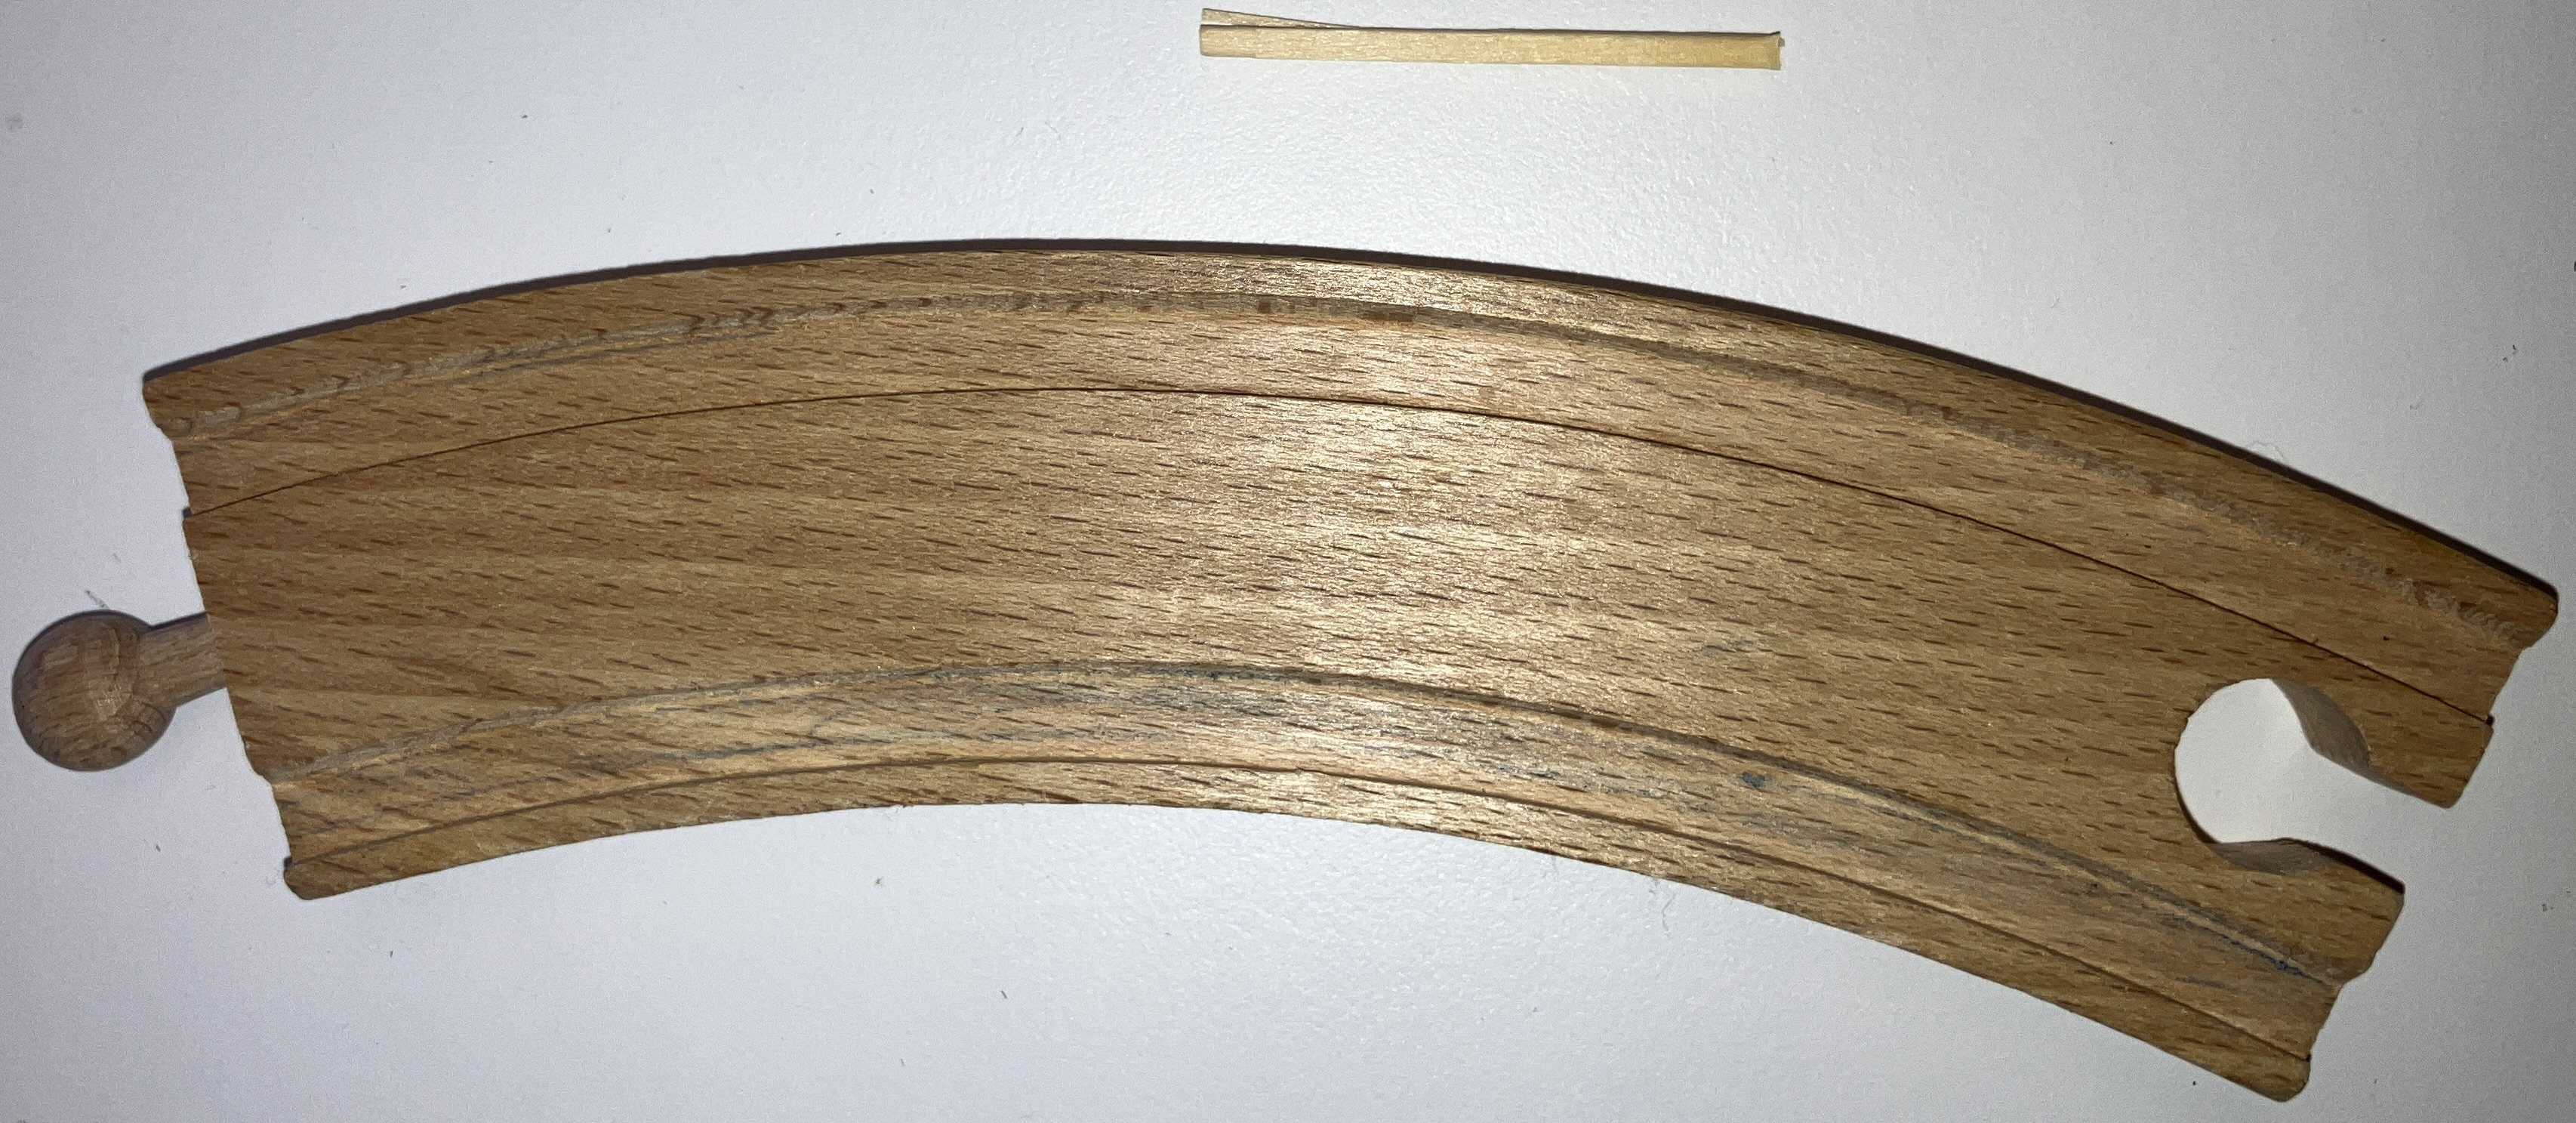
\includegraphics[angle=90, height = 0.9\textheight]{figures/brio_matsticka.JPG}
    \end{columns}
    }
}

\handoutnoteslide

\frame{
    \frametitle{Första uppgiften}
    {\Large
    \begin{columns}
        \column{0.6\textwidth}
        Mät längden på rälsen i enheten ''mätstickor''.\\
        \vspace{5mm}
        Gör allt individuellt (inte titta på någon annan)
        \begin{itemize}
            \item Bestäm bäst mätmetod. Skriv upp hur ni gör!
            \item Mät i hela stickor och tiondelsstickor.
            \item Spara resultatet och meddela mig
        \end{itemize}
    
        \column{0.4\textwidth}
        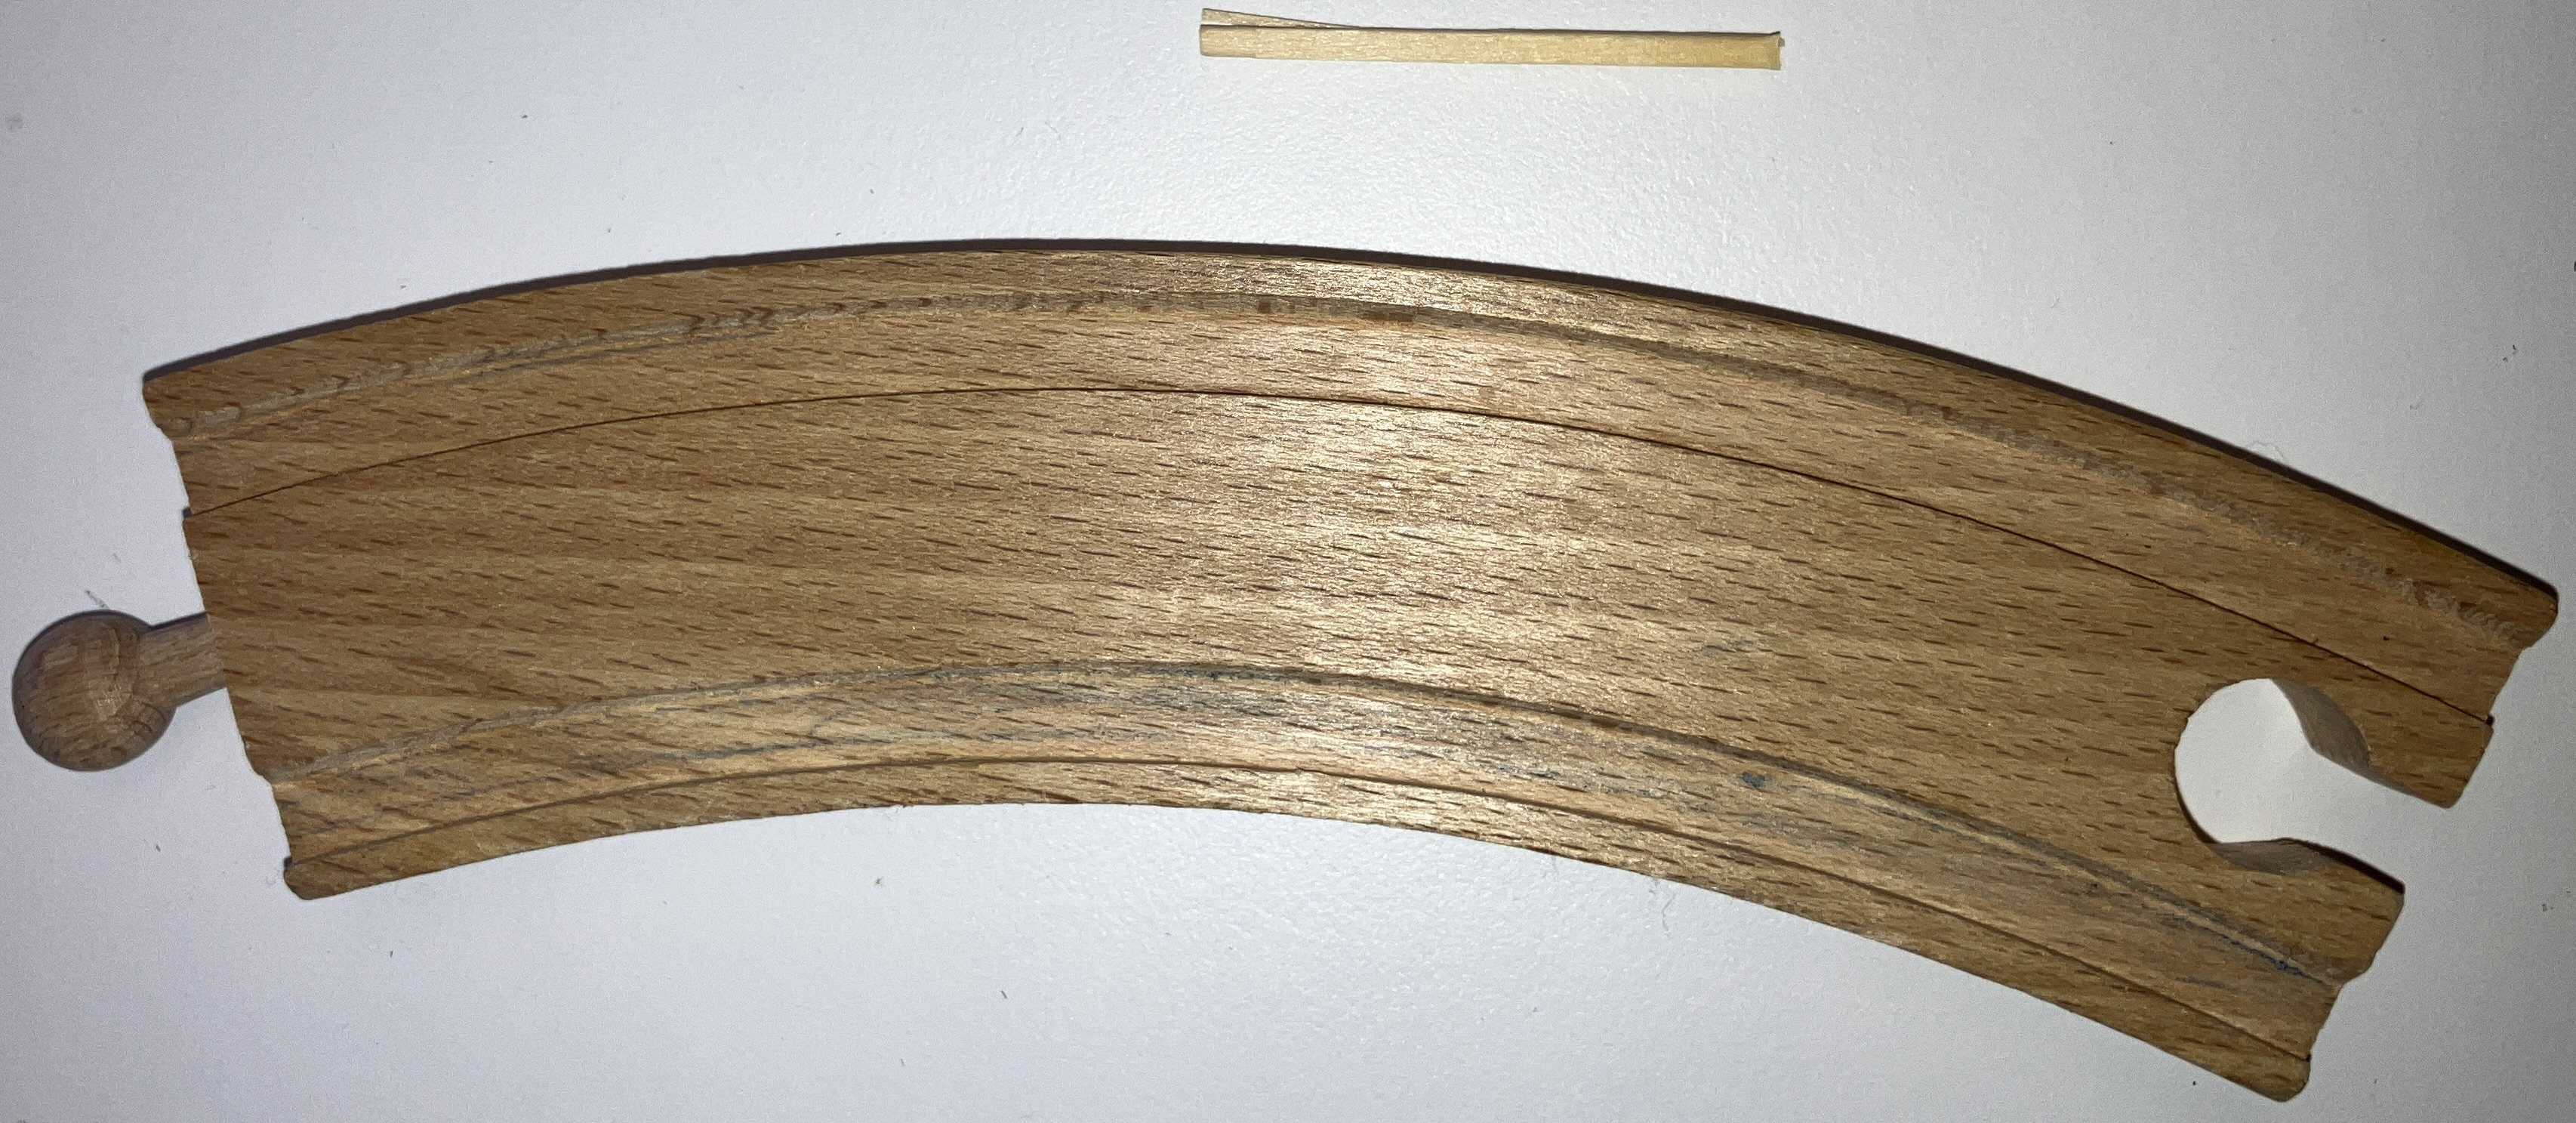
\includegraphics[angle=90, height = 0.9\textheight]{figures/brio_matsticka.JPG}
    \end{columns}
    }
}

\handoutnoteslide

\frame{
\frametitle{Medelvärde och kalibrering}
\centering
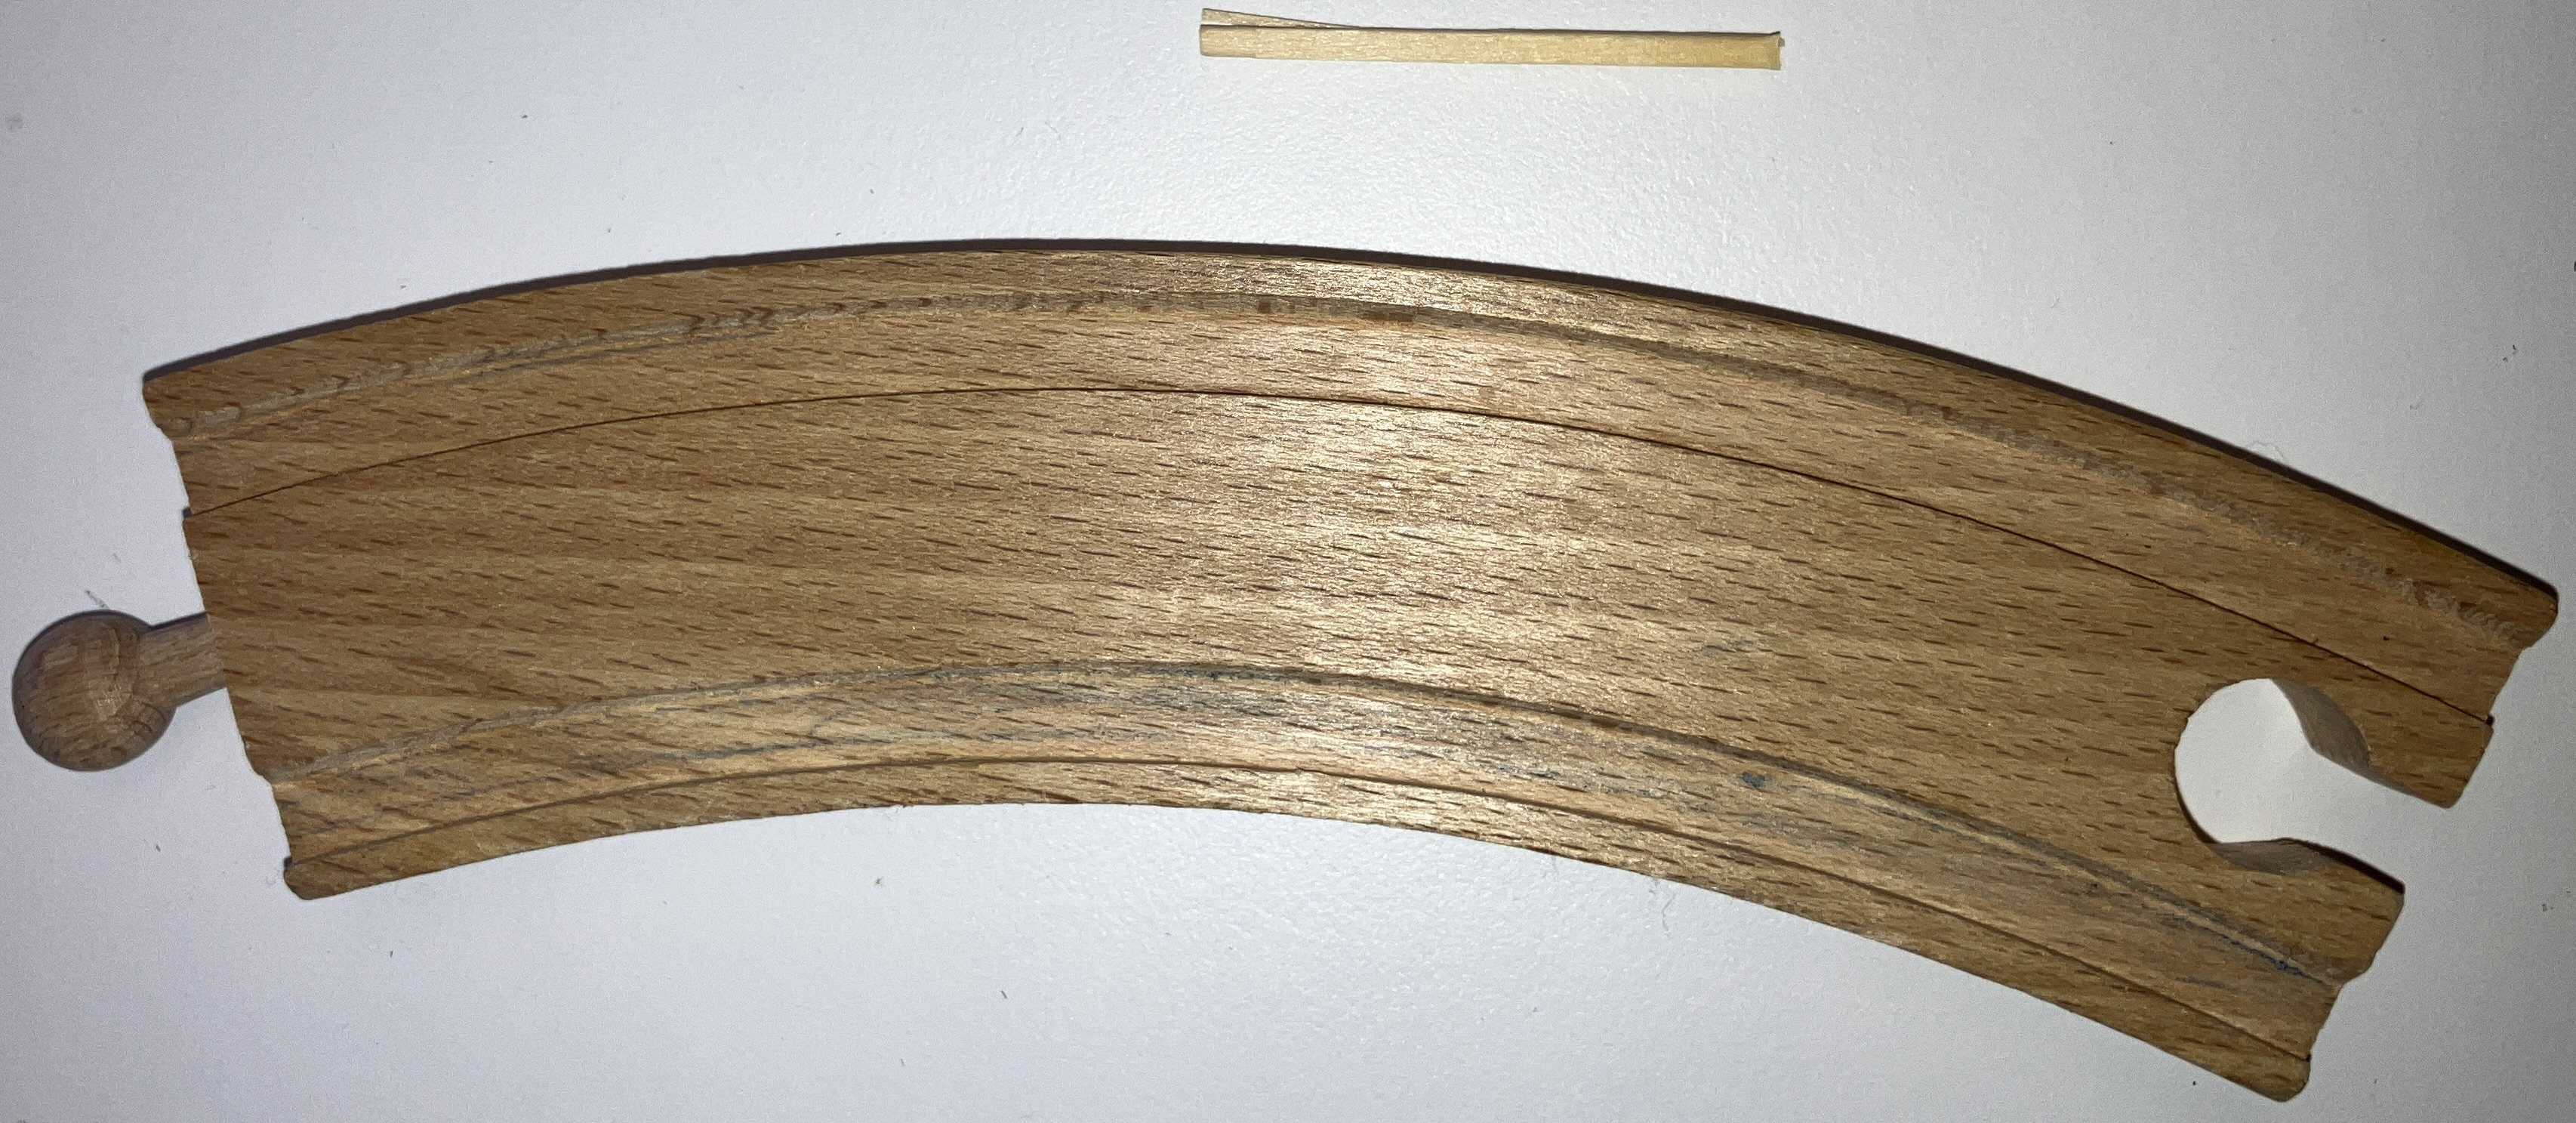
\includegraphics[width=0.8\textwidth]{figures/brio_matsticka.JPG}\\
Medelvärdet är:
\[\bar{x}=\frac{x_1 + x_2 + x_3 + \ldots + x_n}{n}=\]
\onslide<2->{
    Hur noggranna är era mätstickor?
}
}

\handoutnoteslide

\begin{frame}
\frametitle{Mätfel -- noggrannhet}
    \resizebox{!}{0.9\textheight}{
    \begin{tikzpicture}
		\begin{axis}[
			xlabel={Mätvärde (t.ex. figurhöjd)},
			ylabel={Sannolikhetsdensitet},
            axis lines = left,
			width=80mm,
            xmax = 8,
            xmin = -4,
            ymax = 150,
            xtick=\empty,
            ytick=\empty,
			every axis y label/.style={
            at={(ticklabel cs:0.5)},rotate=90,anchor=near ticklabel,},
			every axis x label/.style={
            at={(ticklabel cs:0.5)},anchor=near ticklabel,},
			]
			\addplot [hist={bins=10}] table [col sep=comma] {../dag01/data/legofigurdata_20240811.csv} ;
            	
            	\draw[ultra thick, red] (axis cs:3.75, 0) -- (3.75, 150) node[below, black] {Uppmätt} ;             	
            	
            	\draw[<->, ultra thick, dashed] (axis cs:2,25) -- (5.5,25) node[midway, above] {Precision} ;
            	
            	\draw[ultra thick, red] (axis cs:-1.1, 0) -- (-1.1, 150)  node[below, black] {''Sant''};

            	\draw[<->, ultra thick, dashed] (axis cs:-1.1,100) -- (3.75,100) node[midway, above] {Noggrannhet} ;
		\end{axis}
	\end{tikzpicture}
	} % resizebox
\end{frame}

\handoutnoteslide

\frame{
    \frametitle{}
    {\huge 
    Nu borde ni ha en bra motivering för:
    \begin{itemize}
        \item Mätstandarder (arbetsordrar)
        \item Kalibrering
    \end{itemize}
    }
}

\handoutnoteslide

\mode<beamer>{
    \frame{
        \frametitle{}
        {\Huge Dags att komma till ström!}
    }
}

%%--------------------------------------------------
%% Ny frame
%%--------------------------------------------------
\begin{frame}[fragile]{Ström - vad är det?}
    \begin{columns}
    \begin{column}{0.5\textwidth}
        \begin{block}{(Gammal) definition på ström}
            Två oändligt långa, parallella ledare \qty{1}{\m} isär som påverkar varandra med \qty{0.2}{\micro\N} per meter bär strömmen \qty{1}{\A}.
        \end{block}
        (2019 byttes denna definition.)
    \end{column}
    \begin{column}{0.5\textwidth}
            %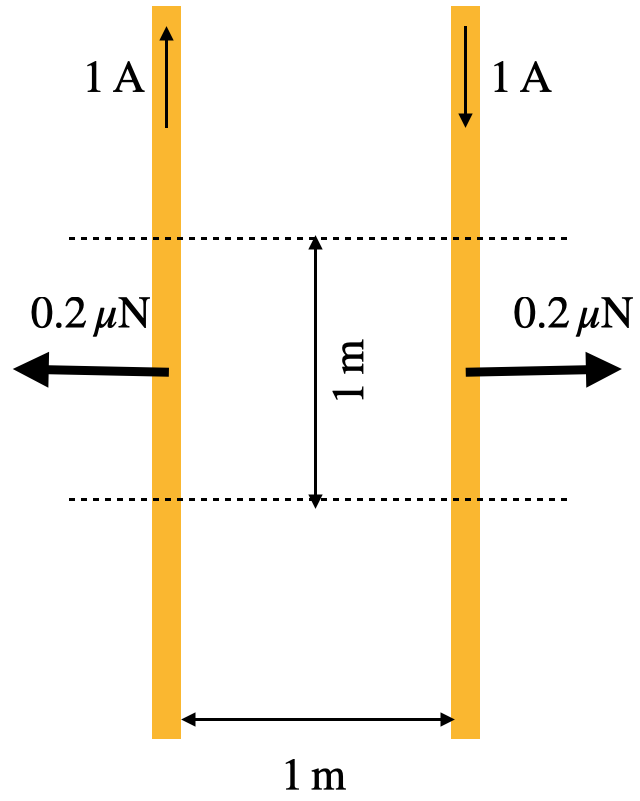
\includegraphics[width = \textwidth]{figures/stromdef.png}\\
        \begin{tikzpicture}[
    x=2cm, y=2cm,
    >={Latex[length=4pt,width=4pt]},
    every node/.style={font=\large, inner sep=0pt},
    force/.style={
        >={Latex[length=10pt,width=10pt]},
        line width=2.5pt
    }
]
    % Vertical conductors
    \fill[orange!80!yellow] (1.115,0) rectangle (1.280,4.165);
    \fill[orange!80!yellow] (2.815,0) rectangle (2.980,4.165);

    % Current arrows
    \draw[->, line width=0.6pt]
        (1.195,3.465) -- (1.195,4.045);
    \node[anchor=east] at (1.080,3.755) {$1\,\mathrm{A}$};

    \draw[->, line width=0.6pt]
        (2.895,4.045) -- (2.895,3.465);
    \node[anchor=west] at (3.045,3.755) {$1\,\mathrm{A}$};

    % Dashed reference lines
    \draw[dash pattern=on 1.5pt off 2pt, line width=0.6pt]
        (0.640,2.840) -- (3.490,2.840);
    \draw[dash pattern=on 1.5pt off 2pt, line width=0.6pt]
        (0.640,1.355) -- (3.490,1.355);

    % One-metre length
    \draw[<->, line width=0.6pt]
        (2.045,1.310) -- (2.045,2.865);
    \node[rotate=90] at (2.225,2.095) {$1\,\mathrm{m}$};

    % Repulsive forces
    \draw[force, ->]
        (1.205,2.080) -- (0.325,2.100);
    \node at (0.770,2.405) {\qty{0.2}{\micro\N}};

    \draw[force, ->]
        (2.900,2.080) -- (3.785,2.100);
    \node at (3.515,2.405) {\qty{0.2}{\micro\N}};

    % Horizontal separation arrow
    \draw[<->, line width=0.6pt]
        (1.280,0.4) -- (2.835,0.4) node[midway, above, yshift=0.2cm] {$1\,\mathrm{m}$};
\end{tikzpicture}
    \end{column}
    \end{columns}
\end{frame}

\handoutnoteslide

%%--------------------------------------------------
%% Ny frame
%%--------------------------------------------------
\begin{frame}[fragile]{Ström och laddning}
    \begin{center}
        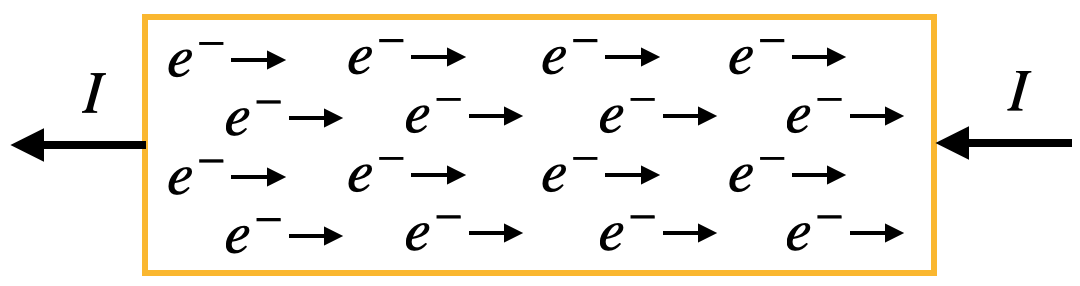
\includegraphics[width = 0.7\textwidth]{figures/stromdef2.png}\\       \begin{block}{Praktisk definition på ström}
        1 Coulomb, \qty{1}{\coulomb}, är den laddning som strömmen \qty{1}{\A} transporterar under \qty{1}{\s}.
        \end{block}
    \end{center}
    \begin{itemize}
        \item<2-> Elektronens laddning: $e=\qty{1.602e-19}{\coulomb}$
        \item<3-> \alert{Observera:} Strömmen och elektronerna går åt olika håll!
    \end{itemize}
    \vspace{5mm}
    \begin{columns}
    \begin{column}{0.5\textwidth}
        \onslide<4->{
        \[ I = \frac{\Delta Q}{\Delta t} \]
        }
        \onslide<5->{
        \[ Q = I \Delta t \]
        }
    \end{column}
    \begin{column}{0.5\textwidth}
        \onslide<4->{
        \[ \qty{1}{\A} = \qty{1}{\coulomb/\s} \]
        }
        \onslide<5->{
        \[ \qty{1}{\coulomb} = \qty{1}{\A\s} \,(\unit{\A\hour}) \]
        }
    \end{column}
    \end{columns}
    \vspace{20mm}
\end{frame}

\handoutnoteslide

%%--------------------------------------------------
%% Ny frame -- nytt innehåll HT2024 samt FMTS
%%--------------------------------------------------
\begin{frame}[fragile]{Att driva ström, ledningsförmåga och Ohms lag}
Olika \emph{ledningsförmåga} (material). \\
''Energi'' driver ström, \emph{spänning} $U$ mäts i \emph{Joule/Coulomb}, eller volt, \unit{\V} 
\begin{center}
    \resizebox{0.45\textwidth}{!}{%
        \begin{tikzpicture}[american]
        	\draw (3, 0) to[R=$R$, v=$U$, i=$I$, o-o] (0, 0) ;
        \end{tikzpicture}
    }% resizebox
\end{center}

\begin{columns}
	\begin{column}{0.45\textwidth}
		\begin{itemize}
			\item<2->\alert{Ledningsförmåga} $G=\frac{I}{U}$, mäts i \emph{siemens}, \unit{\siemens}
			\item<3->\alert{Motstånd} $R = \frac{1}{G}$, mäts i \emph{ohm}, \unit{\ohm}. (Grundenheter: \unit{\kg\m\squared\per\s\cubed\per\A\squared}) %\kg\m^2\s^{−3}A^{−2}}$ 
		\end{itemize}	
	\end{column}
	\begin{column}{0.45\textwidth}
		\begin{itemize}
			\item<4->\alert{Ohms lag} {\huge$U=RI$}
			\item<5->Motstånd vanligast, ledningsförmåga förekommer.
		\end{itemize}
	\end{column}
\end{columns}
\end{frame}

\handoutnoteslide

%%--------------------------------------------------
%% Ny frame -- nytt innehåll HT2024 samt FMTS
%%--------------------------------------------------
\frame{
\frametitle{Att driva ström -- krävs energi -- $U=RI$}
    {\Large
    \begin{columns}
        \column{0.6\textwidth}
    Ström är transport av laddningar.
    \onslide<2->{ \[\text{Spänning} = \frac{\text{Effekt}}{\text{Ström}}\]}
    \onslide<3->{ \[\text{Spänning} = \frac{\text{Energi}}{\text{Laddning}}\]}
    \onslide<4->{\huge \[ P = U \cdot{} I \] }
        \column{0.4\textwidth}
    \centering
    \onslide<5->{\qty{75}{\W}\\}
    \onslide<6->{
    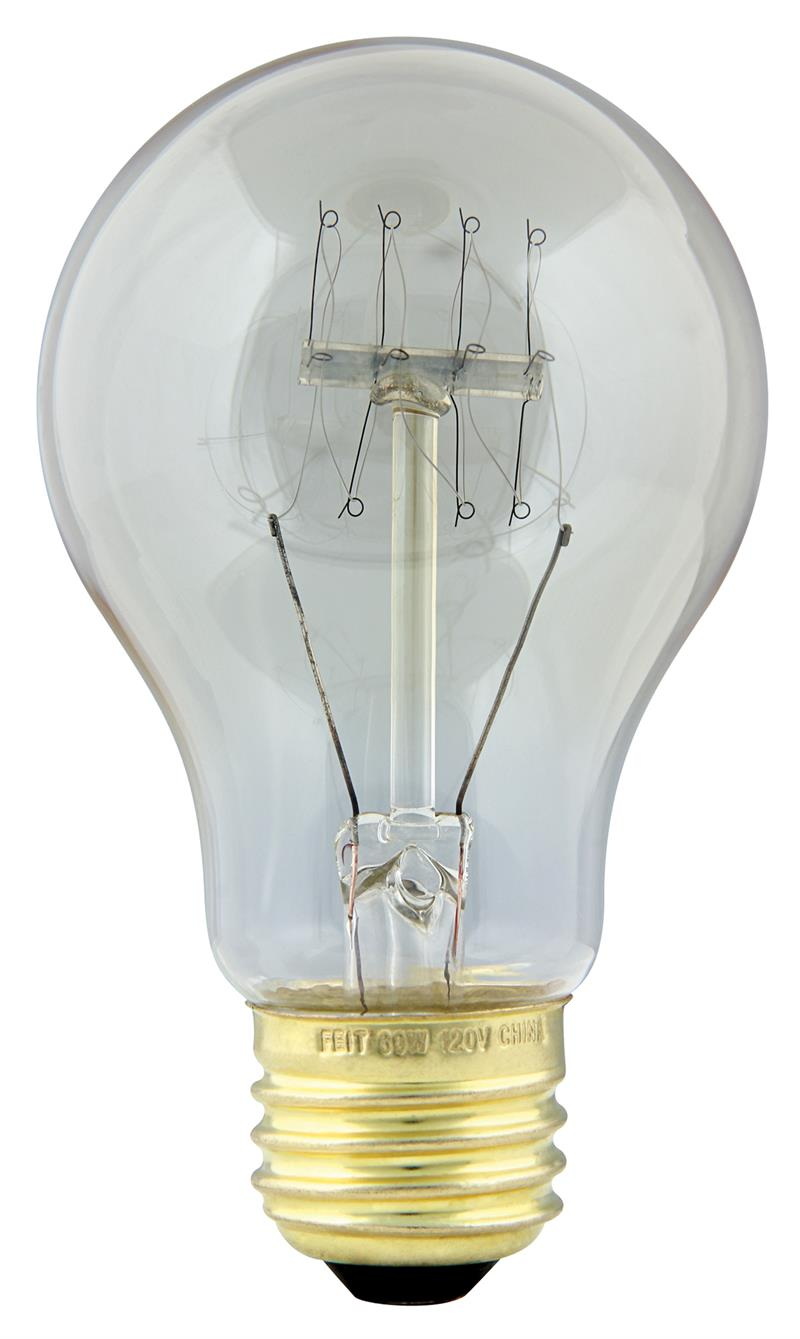
\includegraphics[width=0.75\textwidth]{figures/glodlampa.jpg}
    }
    \end{columns}
    }
}

\handoutnoteslide

\begin{frame}
\frametitle{Ohms lag och resistans}
\begin{center}

\resizebox{0.67\textwidth}{!}{%
    \begin{tikzpicture}[scale = 1, american]
        \draw (0, 0) 
        to[american voltage source=\qty{25}{\V}, invert, *-] (0, 2) 
        -- (2, 2) 
        to[R=\qty{50}{\ohm}, i=$I$] (2, 0) 
        -- (0, 0) 
        node[ground, rotate=-90] {};
    \end{tikzpicture}
} % resizebox

    {\huge Bestäm strömmen $I$ ovan.}
\end{center}
\end{frame}

\handoutnoteslide

\begin{frame}\frametitle{Ohms lag och resistans}
\resizebox{\textwidth}{!}{%
\begin{minipage}{.5\textwidth}
\centering
\begin{tikzpicture}[scale = 1, american]
    \draw (0, 0) 
    node[ground] {}
    to[american voltage source=\qty{25}{\V}, invert] (0, 2) 
    -- (2, 2) 
    to[R=\qty{50}{\ohm}, i=$I$] (2, 0)
    node[ground] {}
    ;
\end{tikzpicture}\\
Bestäm strömmen $I$ ovan.
\end{minipage}}
\end{frame}

\handoutnoteslide

%%--------------------------------------------------
%% Ny frame
%%--------------------------------------------------
\begin{frame}[fragile]{Mer om potential (och nu kretsar)}
  \begin{columns}
    \column{0.3\textwidth}
    \begin{center}
    
\includegraphics[width=0.8\textwidth]{figures/idealledare.png}\\
    \onslide<2->{
      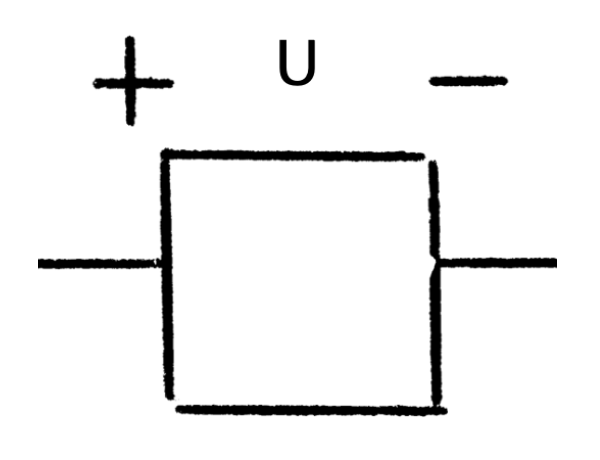
\includegraphics[width=0.8\textwidth]{figures/komponent.png}\\
    }
    \onslide<3->{
      
\includegraphics[width=0.5\textwidth]{figures/jord.png}
    }
    \end{center}
    \column{0.2\textwidth}
    Ideal ledare\\
    \vspace{12mm}
    \onslide<2->{
      Elektrisk komponent\\
    }
    \vspace{12mm}
    \onslide<3->{
      Jord ($V=\qty{0}{\V}$)
    }
    \column{0.5\textwidth}
    \onslide<4->{
      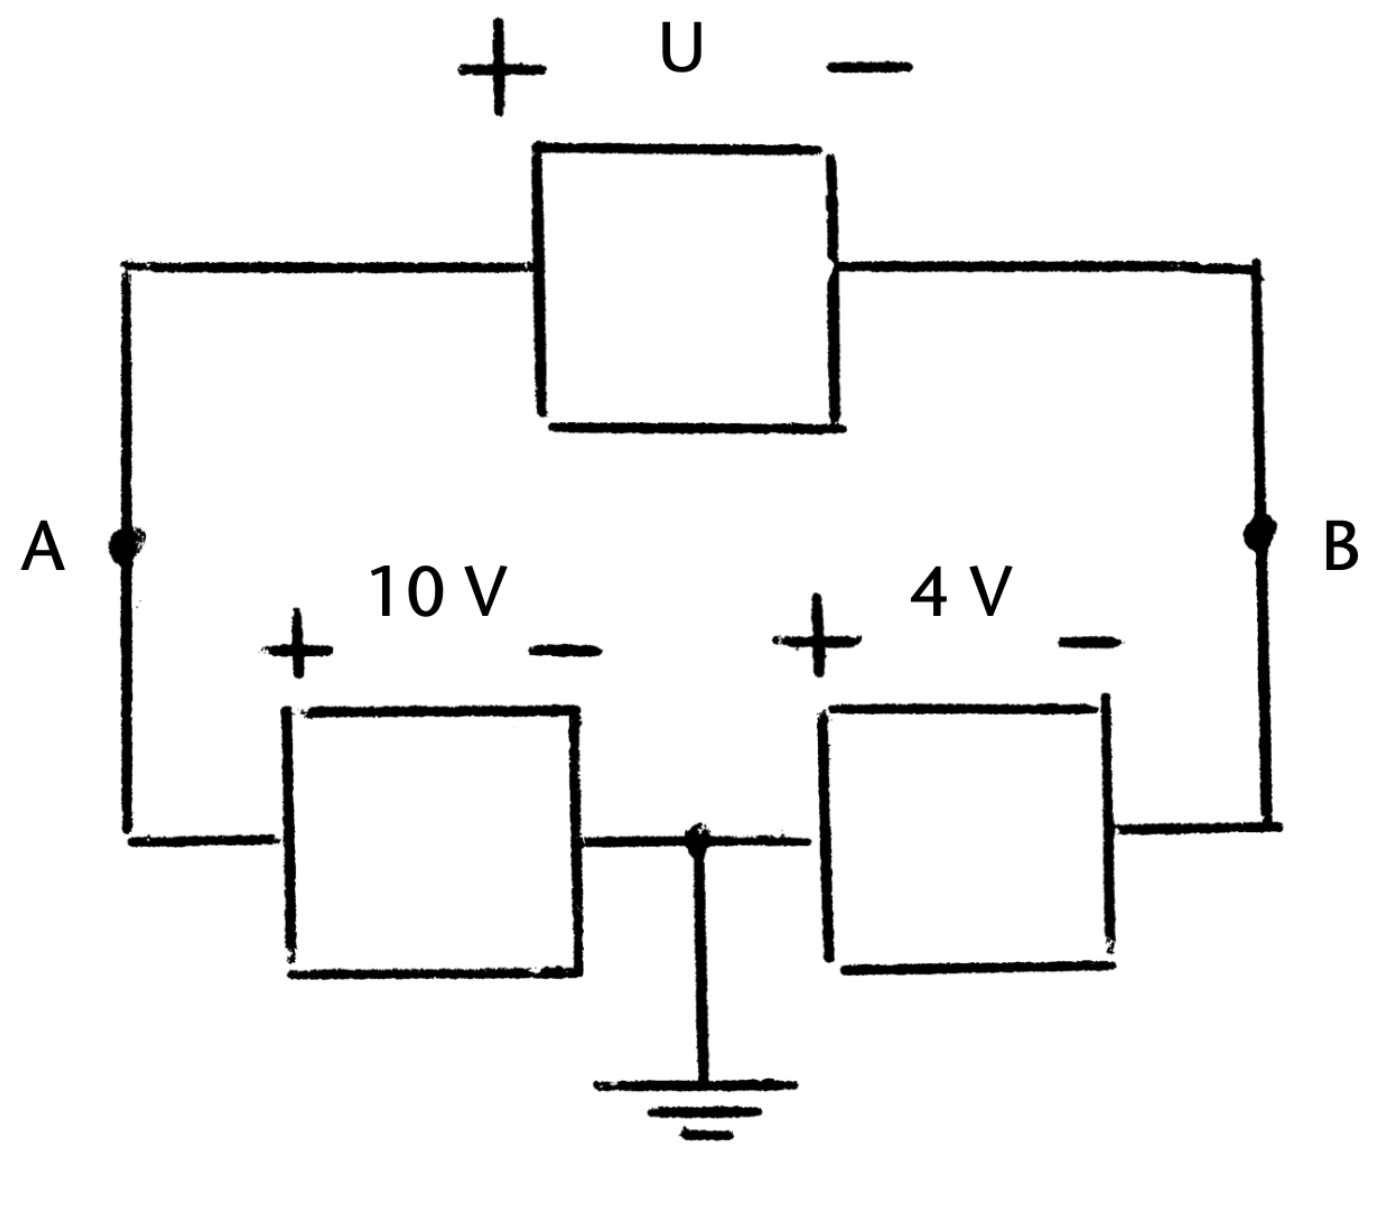
\includegraphics[width=\textwidth]{figures/krets.png}\\
    }
    \onslide<5->{
    Tar ut energi $V<\qty{0}{\V}$, last (\textit{load})\\
    Ger energi $V>\qty{0}{\V}$, källa (\textit{source})
    }
  \end{columns}
\end{frame}

\handoutnoteslide

%%--------------------------------------------------
%% Ny frame
%%--------------------------------------------------
\begin{frame}[fragile]{Mer om potential (och nu kretsar)}
  \begin{columns}
    \column{0.6\textwidth}
    \Large
      Potentialvandring\\ \vfill
      \onslide<2->{
        $V_{\mathrm{jord}}\equiv 0$ \hspace{2mm}
        
\includegraphics[width=0.1\textwidth]{figures/jord.png} \hspace{2mm}
        Jord!\\ \vfill
      }
      
      \onslide<3->{
        $V_B=\qty{0}{\volt}-\SI{4}{\volt}$\\ \vfill
      }
      
      \onslide<4->{
        $V_A=\qty{0}{\volt}+\SI{10}{\volt}$\\ \vspace{5mm}
      }
    \onslide<5->{\Large
      Spänning (voltmeter) } 
    
      
    \column{0.4\textwidth}
    \onslide<1->{
      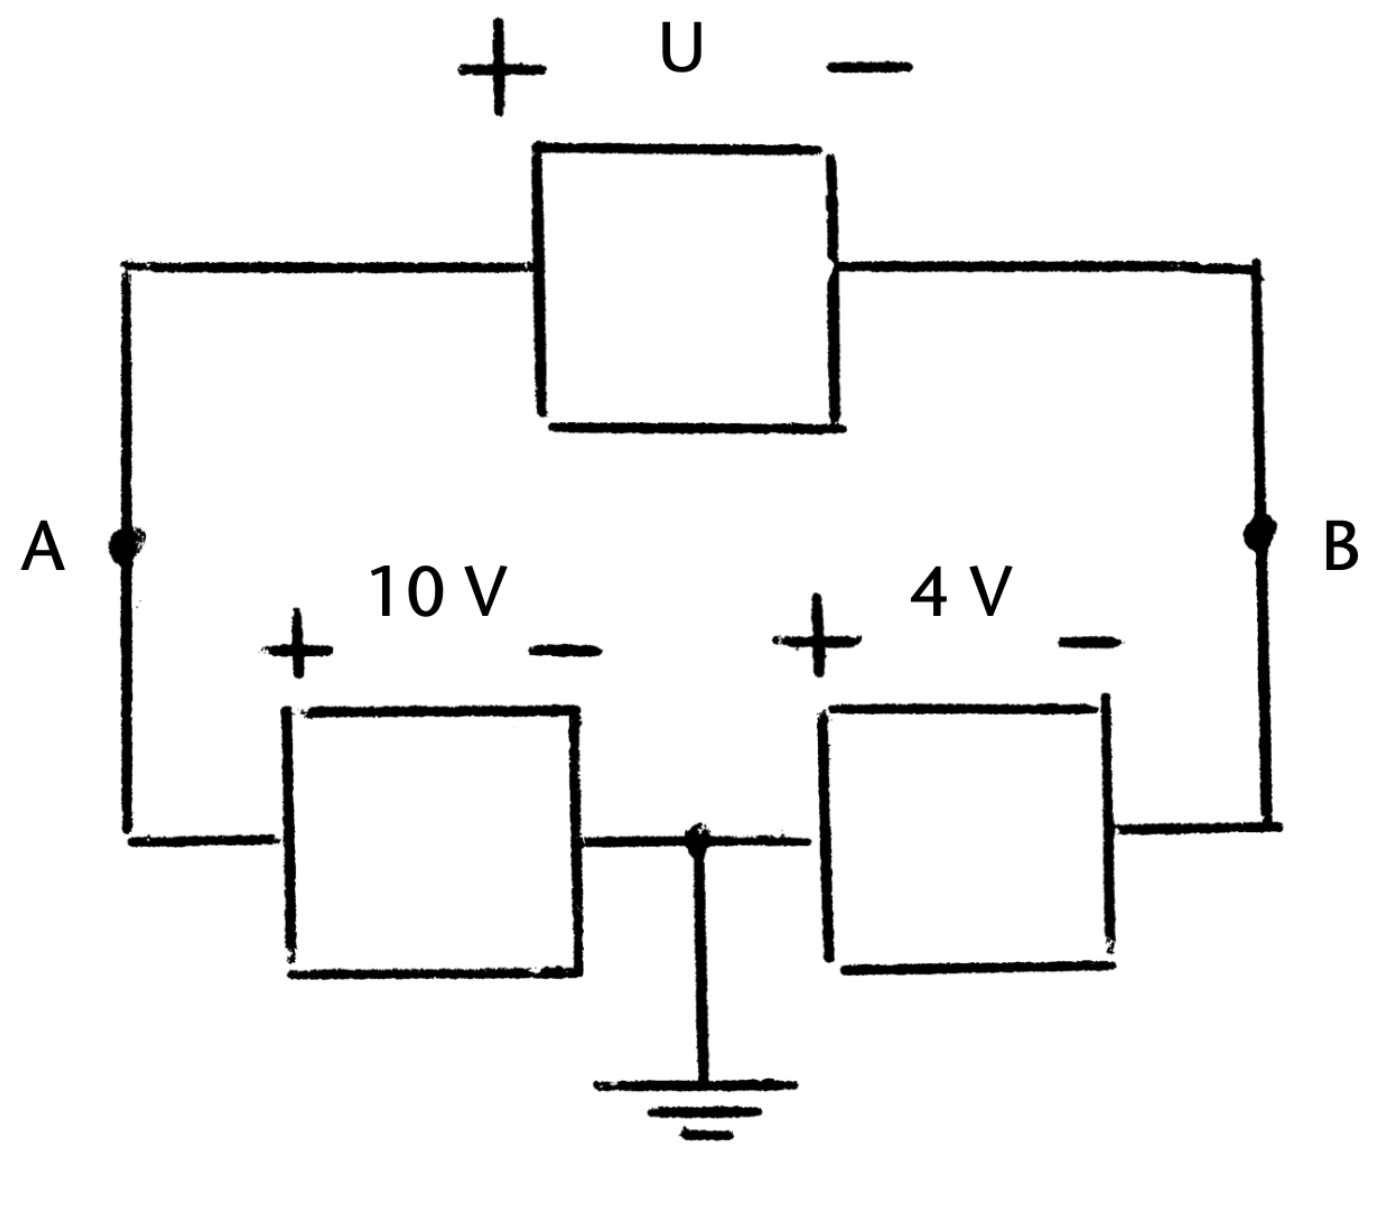
\includegraphics[width=\textwidth]{figures/krets.png}
    }
  \end{columns}
  {\huge
  \onslide<6->{
        $U_{AB}=V_A-V_B$} \onslide<7->{ $ =\qty{10}{\volt}-\left(-\qty{4}{\volt}\right)
        =\qty{14}{\V}$
    }}
\end{frame}

\handoutnoteslide

\descriptionslide{figures/kvl-exempel.png}{0.75}{Bestäm $U_1$}{}

\handoutnoteslide

%%--------------------------------------------------
%% Ny frame
%%--------------------------------------------------
\begin{frame}[fragile]{Strömmar i kretsar}
  \begin{columns}
    \column{0.4\textwidth}
    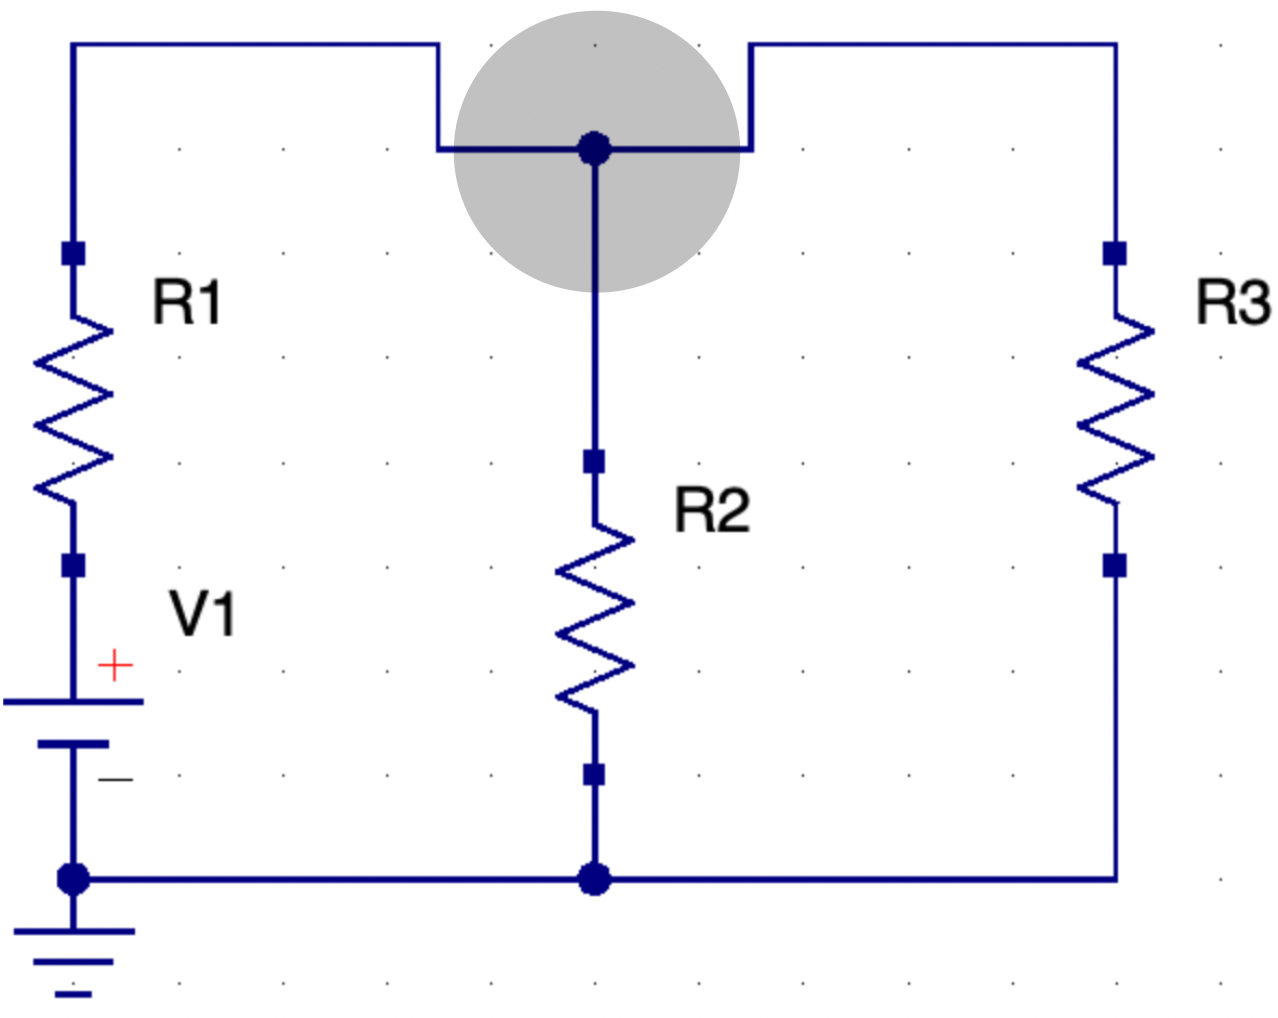
\includegraphics[width=\textwidth]{figures/krets_qucs.png}
    \column{0.6\textwidth}
    \Large
    \begin{itemize} % specificera label för
    \item<1-> Laddning \alert{bevarad.}
    \item<1-> Strömmar går vidare (eller inte alls).
    \item<3-> \alert{\emph{In mot}} knut -- positiva
    \item<3-> \alert{\emph{Ut från}} knut -- negativa
    \end{itemize}
    \onslide<2->{
      $\sum I_i =0$
    }
    
  \end{columns}
%  \vspace{5mm}
  \begin{columns}
  	\column{0.1\textwidth}
    \column{0.4\textwidth}
    \onslide<2->{
      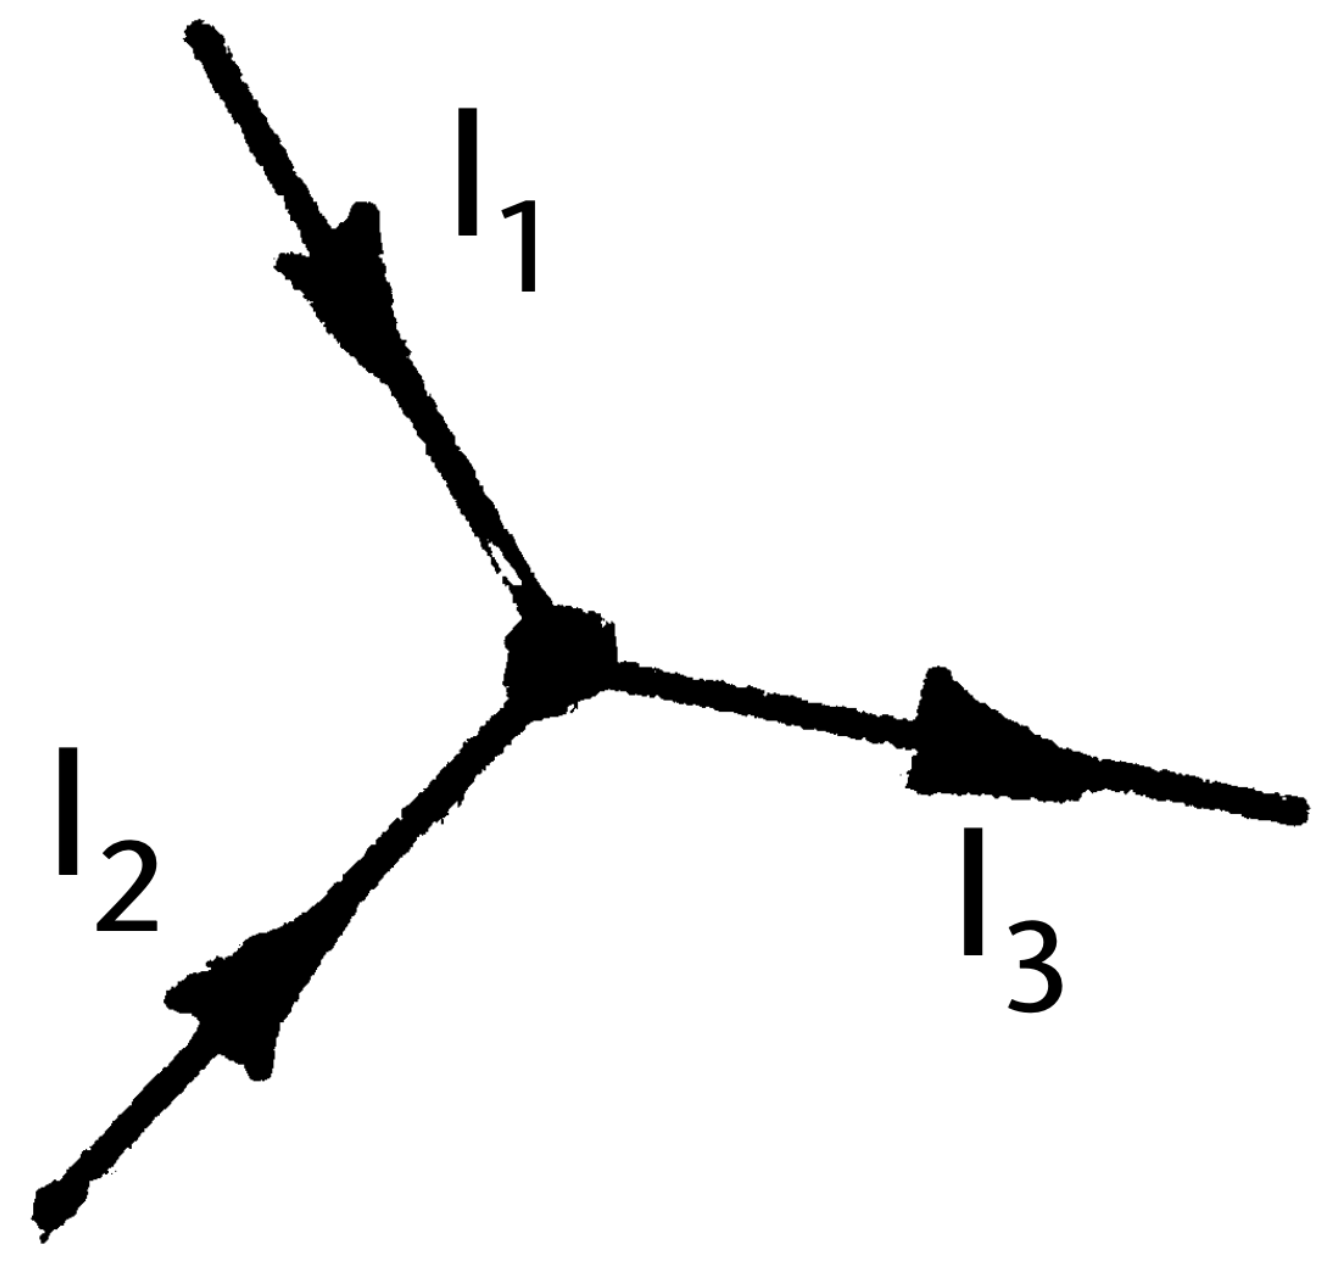
\includegraphics[width=0.7\textwidth]{figures/stromknut_arne.png}
    }
    \column{0.5\textwidth}
    \Large
    \onslide<4->{
      \[I_1+I_2-I_3=0\]
    }
  \end{columns}
\end{frame}

\handoutnoteslide

\descriptionslide{figures/kcl-exempel.png}{0.5}{Bestäm $I$}{}

\handoutnoteslide

%% Nytt stuff HT2026 - introlabben från ET2010 som uppvärmning.

\mode<beamer>{
% Manualframsidor
\begin{frame}[plain]
  \centering
  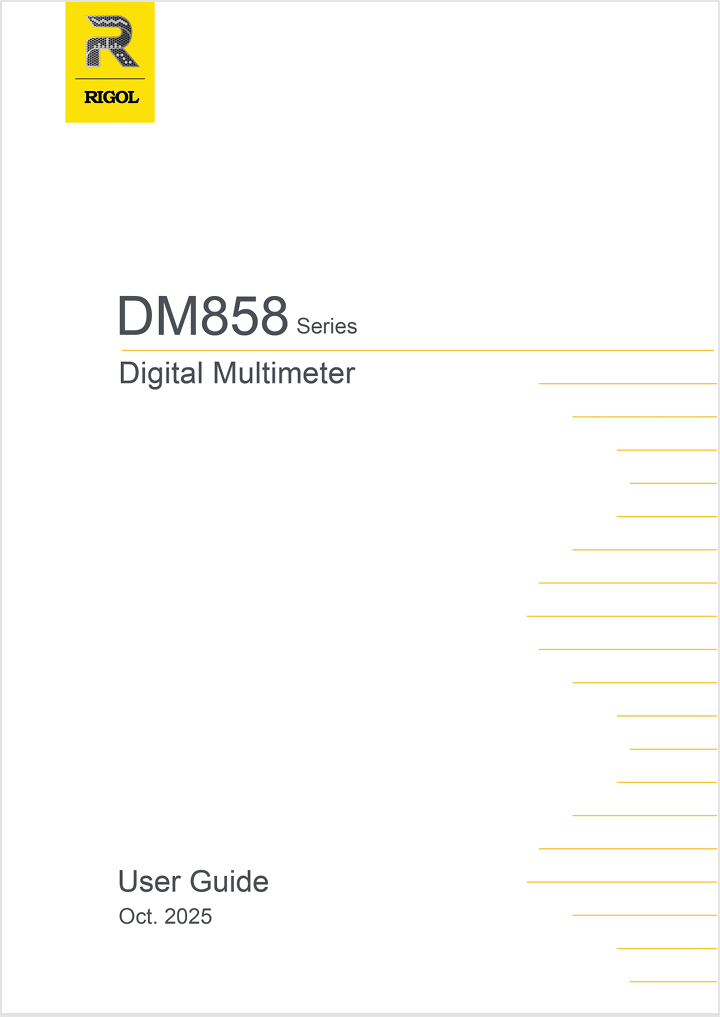
\includegraphics[height=\paperheight]{figures/dm858_manual_1stpage.png}\hfill
  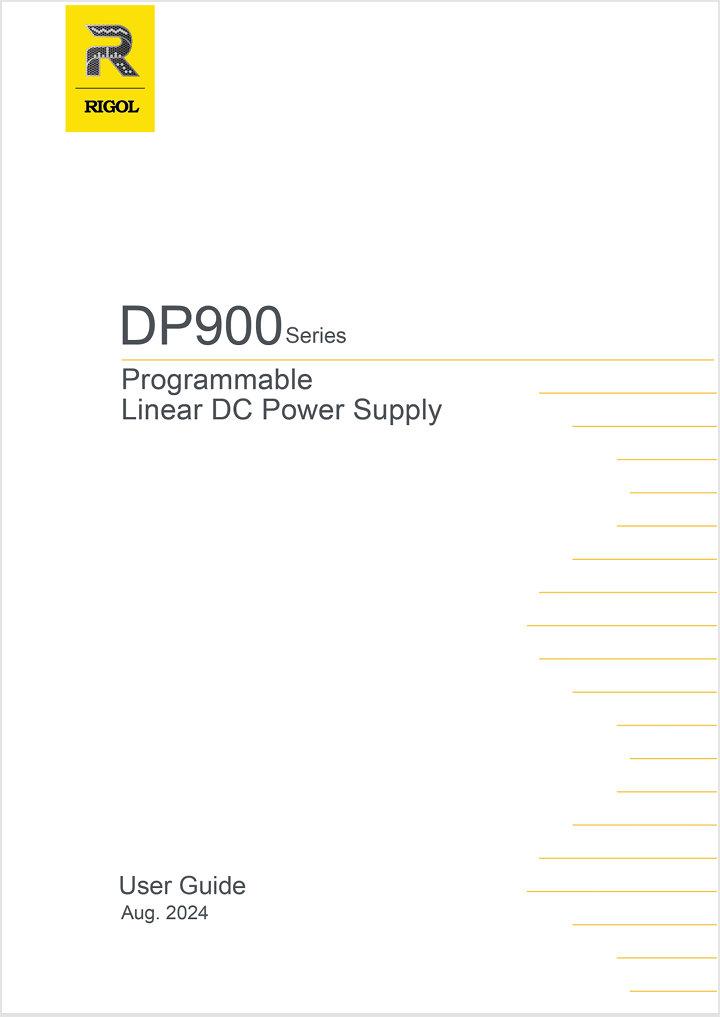
\includegraphics[height=\paperheight]{figures/dp900_manual_1stpage.png}
\end{frame}


% Manualframsidor
\begin{frame}[plain]
  \centering
  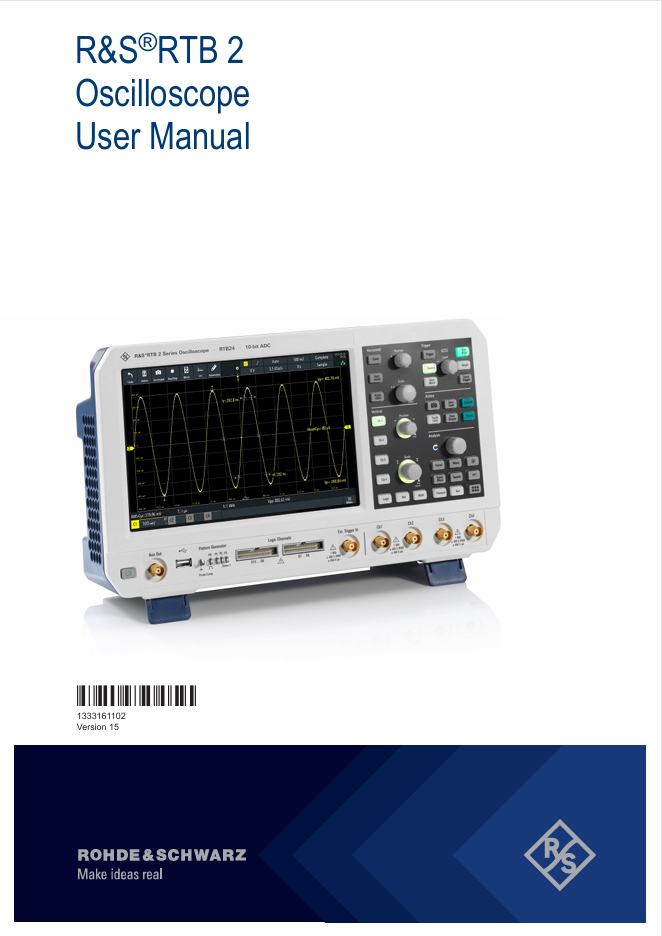
\includegraphics[height=\paperheight]{figures/rohdemanual.png}\hfill
  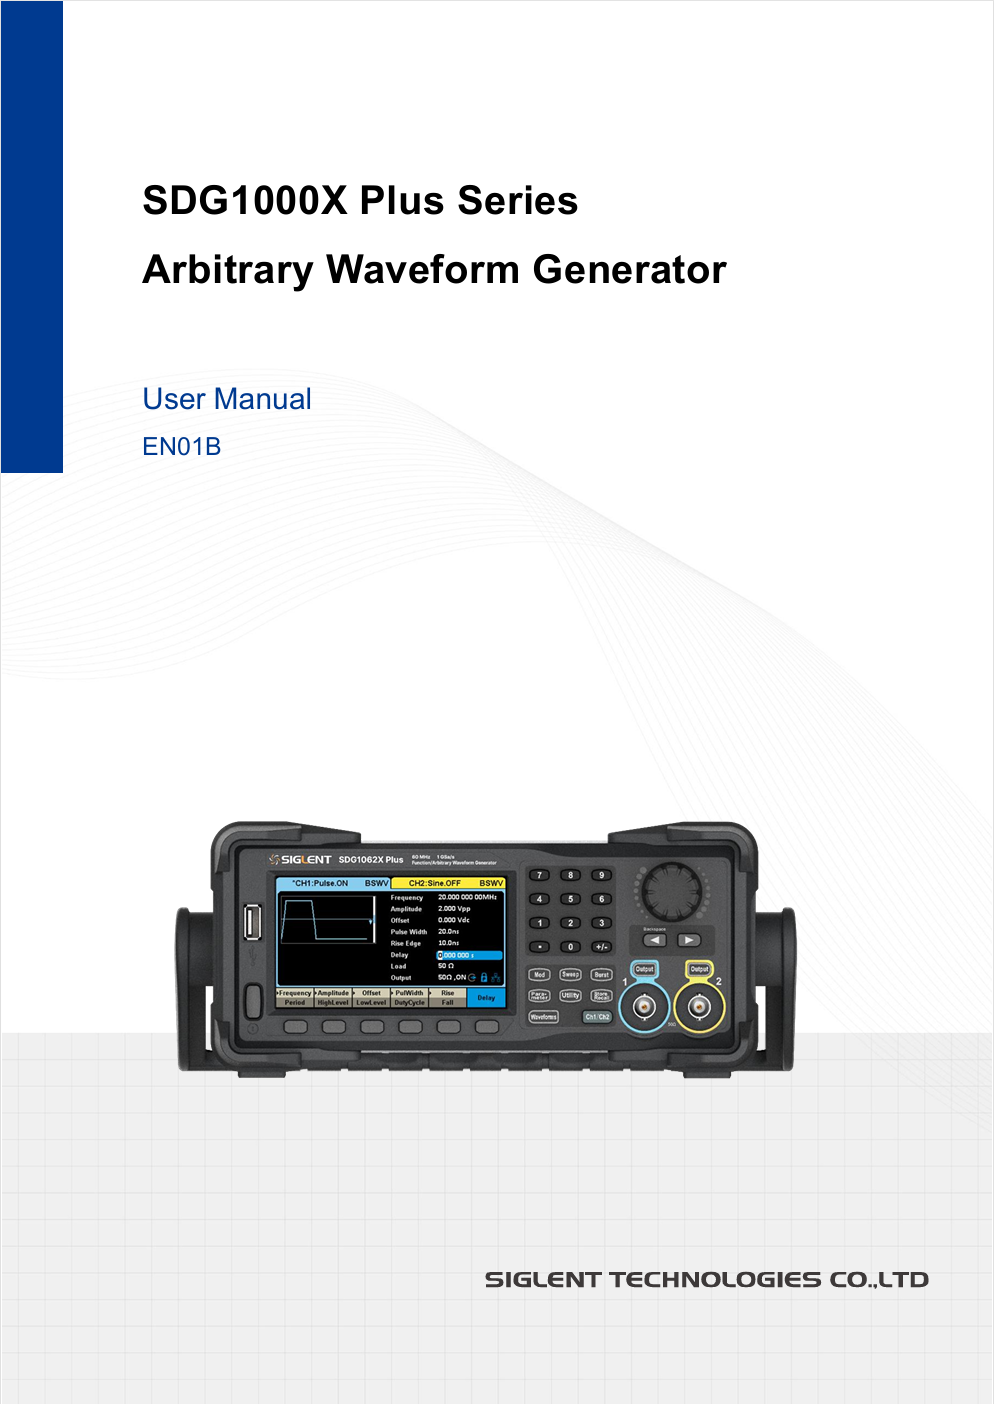
\includegraphics[height=\paperheight]{figures/siglentmanual.png}
\end{frame}
} % mode beamer slut


% banankontakt och hemma-multimeter
\begin{frame}[plain]
  \centering
  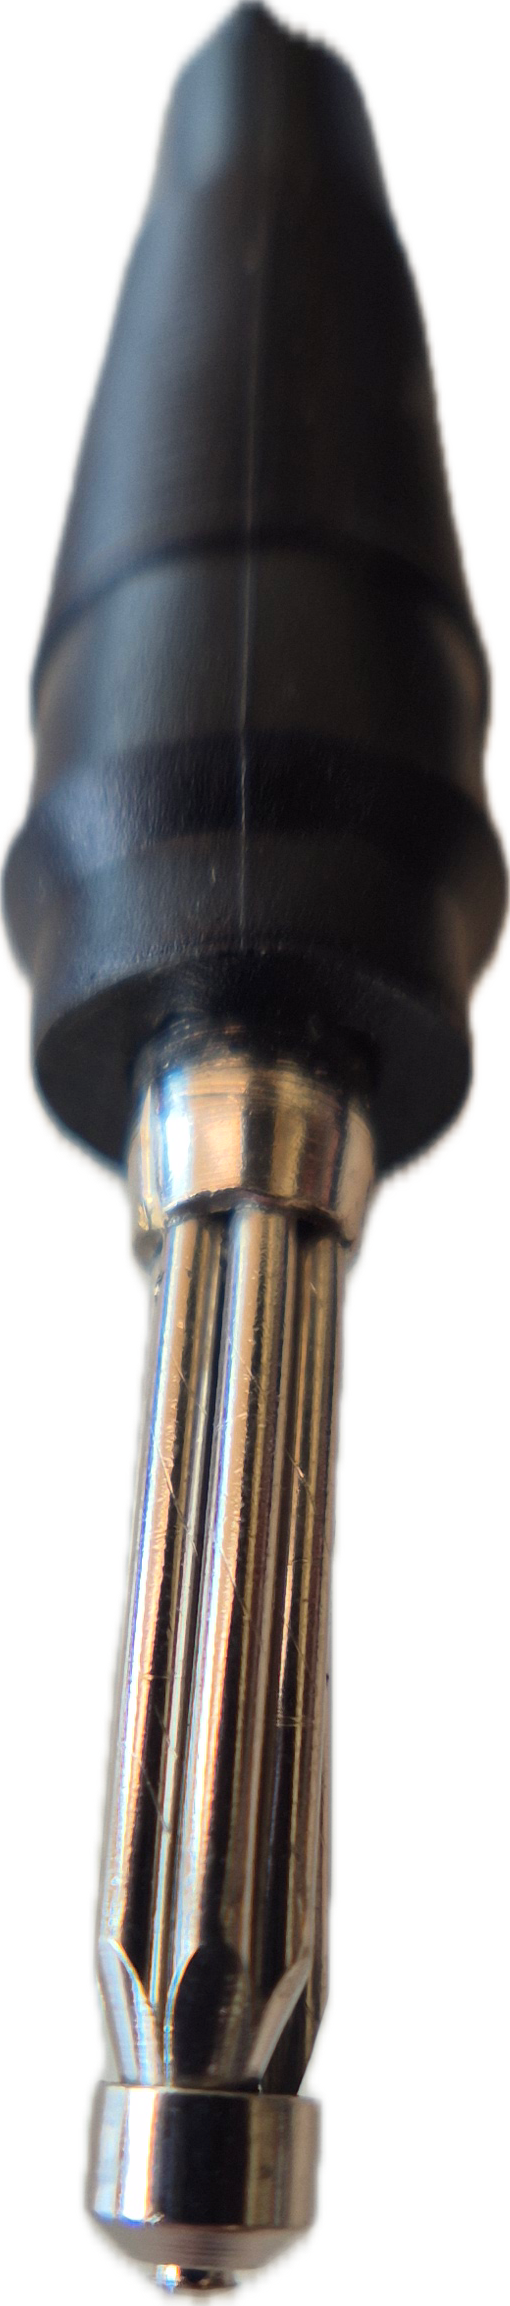
\includegraphics[height=\paperheight]{figures/banankontakt_ny.png}\hfill
  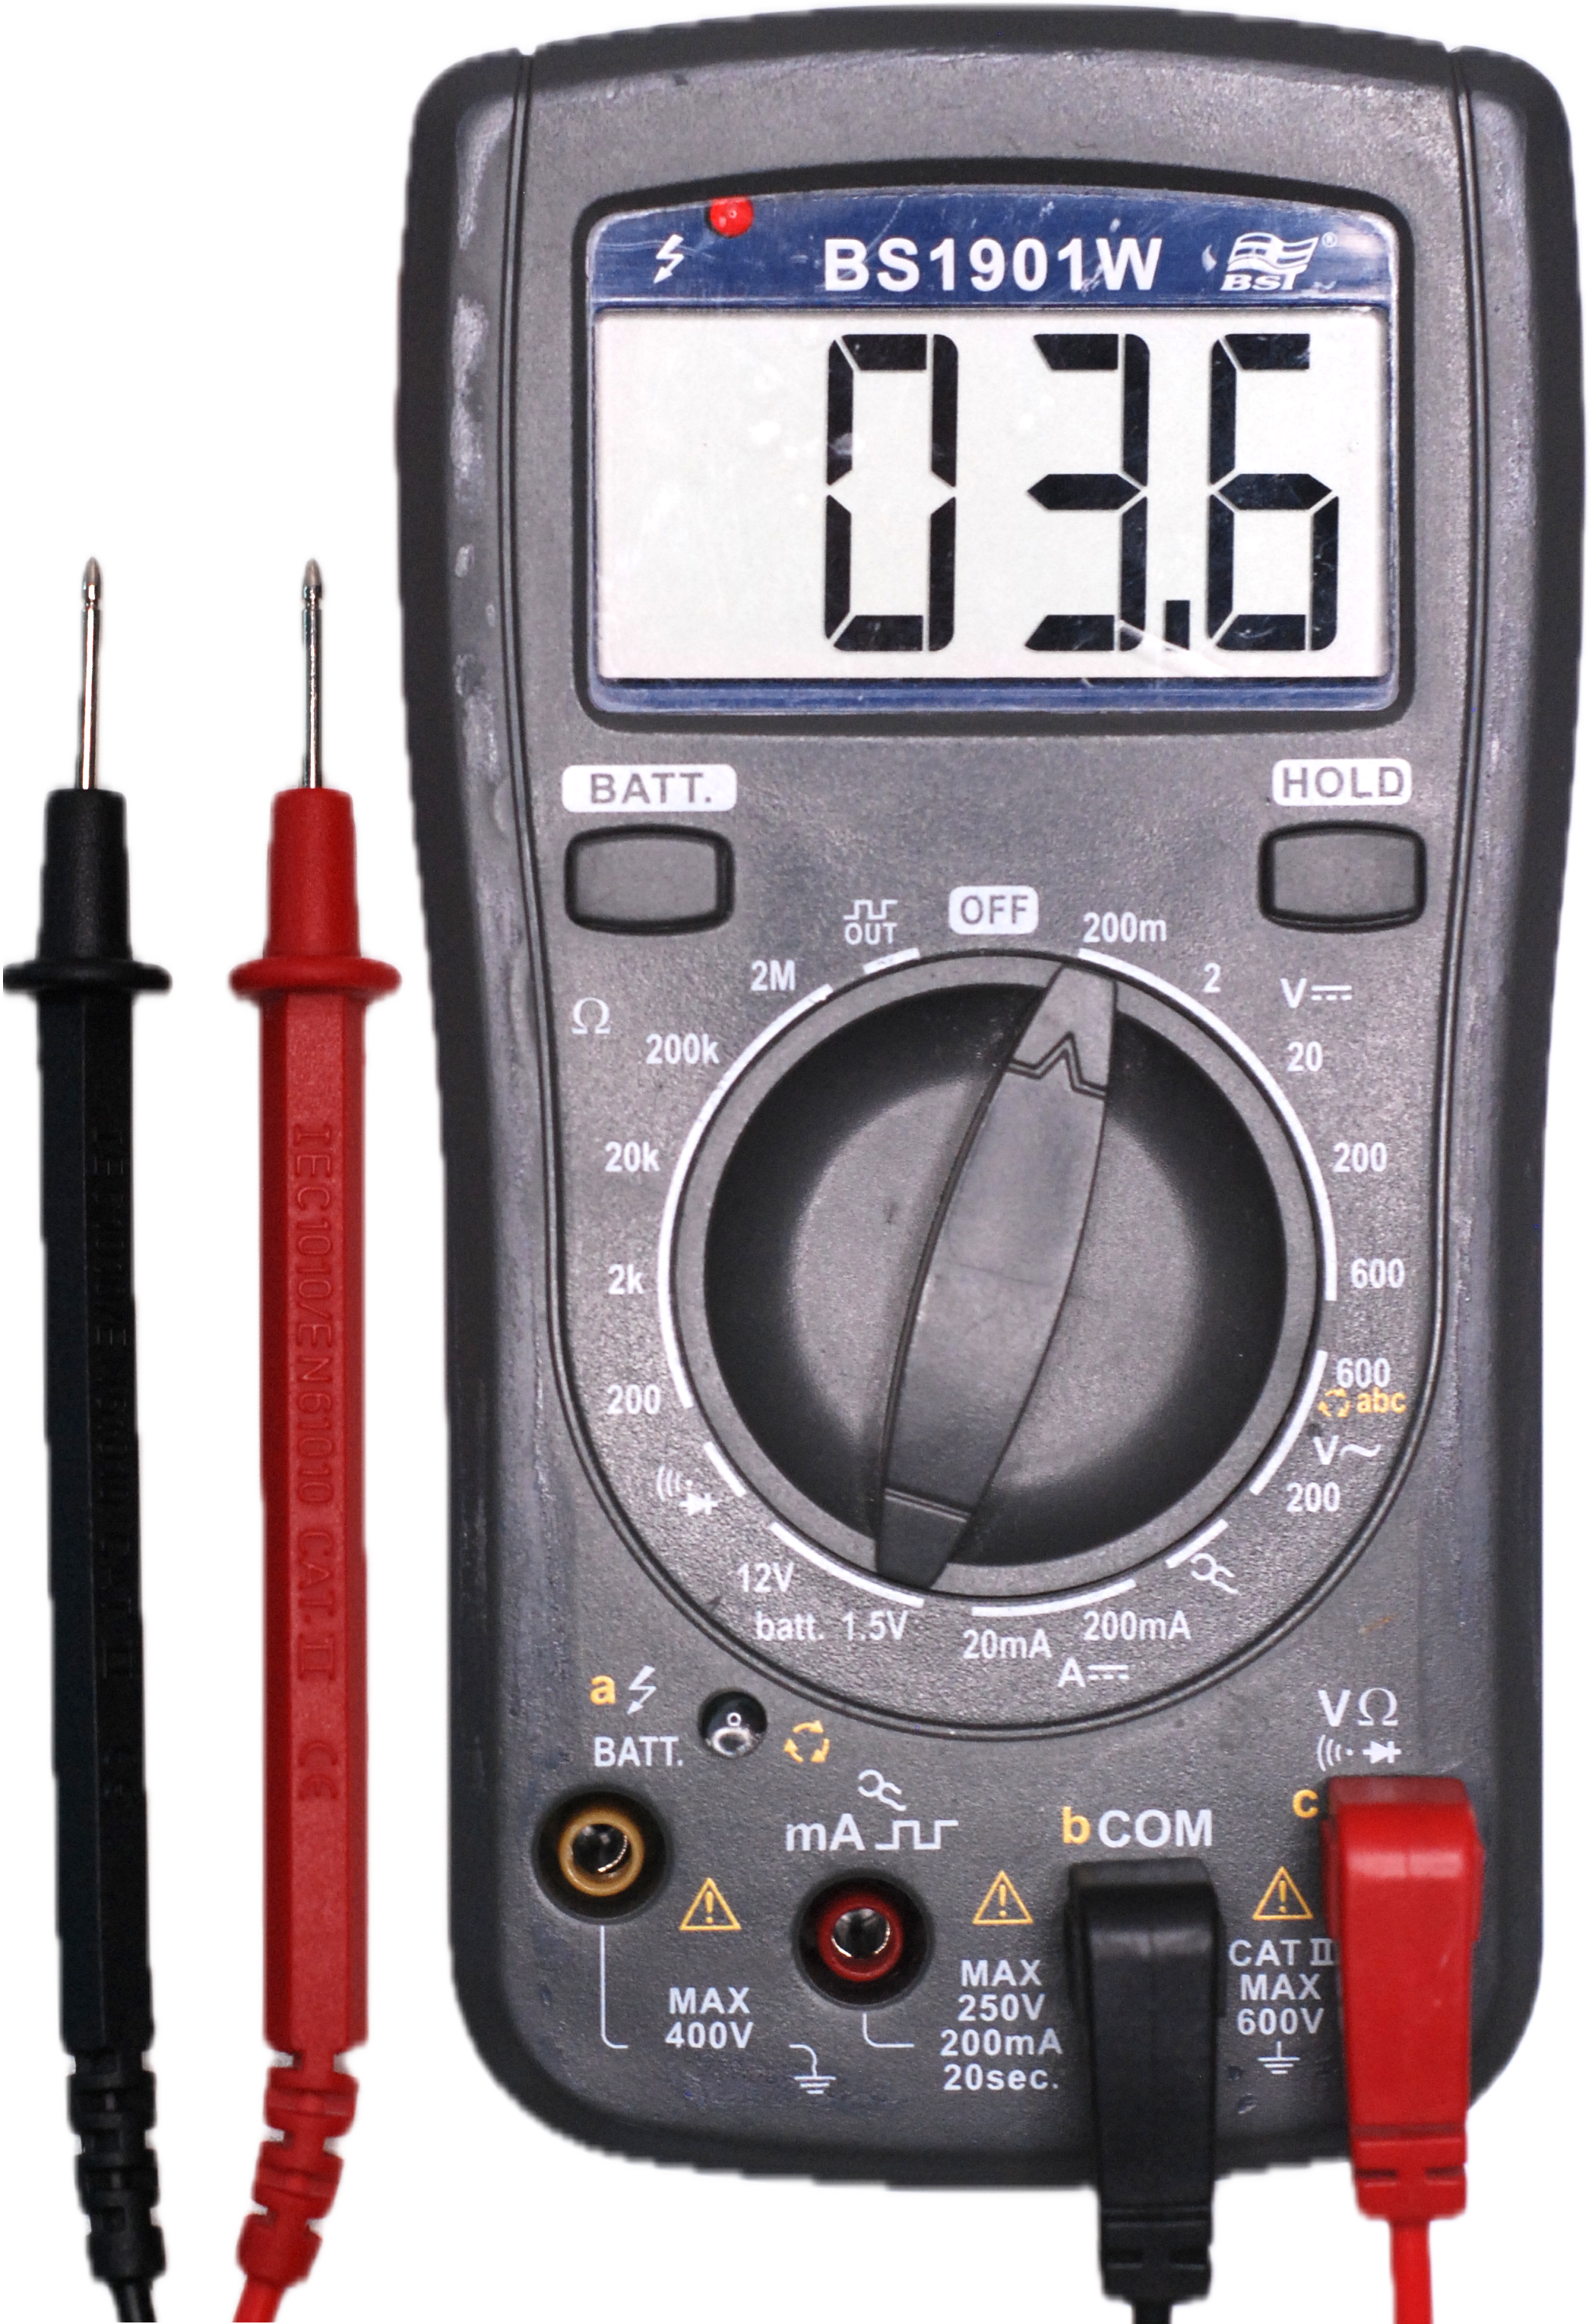
\includegraphics[height=\paperheight]{figures/c04_dmm-3.6mA_prob.png}
\end{frame}

\handoutnoteslide

\descriptionslide{figures/rigol_multimeter.png}{1}
    {Bänkmultimeter Rigol DM838E}{}

\descriptionslide{figures/dm858_sketch.png}{0.9}{}{}

\descriptionslide{figures/rigol-input-voltage.png}{0.5}
  {Koppla så här för att mäta spänning eller motstånd med Rigol DM838E. Ofarligt!}{}


\mode<beamer>{
  \descriptionslide{figures/rigol_multimeter.png}{0.9}{Mäta spänning.}{
  \ringmarker{red}{0.67}{0.90}{0.45}
}

\descriptionslide{figures/rigol_multimeter.png}{0.9}{Mäta resistans.}{
  \ringmarker{red}{0.78}{0.88}{0.45}
}

\descriptionslide{figures/rigol_multimeter.png}{0.9}{Mäta avbrott, ''pipa'' kretsen.}{
  \ringmarker{red}{0.83}{0.90}{0.45}
}
} % mode beamer ends

\mode<beamer>{
\sectionslide{Nu säger vi alla i kör: \\[5mm] \pause{} Spänningsmätning och motståndsmätning\\[2mm] är relativt säkert.}
\sectionslide{Labbets farligaste djur: Krokodilen!}
} % end mode.

\descriptionslide{figures/c04_krokodilerAlla.png}{1.0}
    {Isolerade och oisolerade krokodilklämmor. \\ 
    Undvik krokodilklämmor om det inte är absolut nödvändigt! \\ 
    Använd \textit{bara} isolerade krokodilklämmor!}{}


\mode<beamer>{
\sectionslide{Kopplingsdäck, demoboard, breadboard.}

\descriptionslide{figures/c04_breadboard_photo.png}{0.9}{Kopplingsdäck, breadboard.}{}

\descriptionslide{figures/breadboard_connections.png}{1}{Kopplingarna \textit{inuti} breadboarden.}{}

\descriptionslide{figures/c04_breadboar_with_resistor.png}{0.9}{Kopplingsdäck med komponent.\\ Komponenter hålls på plats med fjädrar,\\ bara ett ben i varje hål. Testa flytta runt\\ och sätt ut komponenter och \textit{jumper wires}.}{}

\descriptionslide{figures/c04_probeTip.png}{1.0}{Probspets i hål mot komponentben.}{}

\descriptionslide{figures/breadboard_tworesistors.png}{0.8}{Koppla upp två motstånd. Mät motståndet över ena och bägge. Mät kontakt (pip) i raden där bägge är inkopplade.}{}

\descriptionslide{figures/breadboard_circuit_longWires.png}{1}{Koppling med långa jumper wires.}{}

\descriptionslide{figures/breadboard_circuit_shortWires.png}{1}
    {Koppling med korta jumper wires.}
    {
        \ringmarker{red}{0.6}{0.325}{1}
    }

\descriptionslide{figures/fritzing.jpg}{1}{Koppla upp denna kretsen! (Strunta i batterierna.)}{}
} % end beamer mode

\descriptionslide{figures/fritzing.jpg}{2}{Koppla upp denna kretsen! (Strunta i batterierna.)\\Visa Pererik när ni är färdiga, förklara hur strömmen går.}{}

\handoutnoteslide

\mode<beamer>{
%% Power supply och labbmatning
\sectionslide{Labbmatning och labbspänningsaggregat.}
} % end mode

\descriptionslide{figures/dp932e.png}{1.2}{Spänningsaggregat, labbaggregat,\\ \textit{DC Power supply}. Denna har kraft\\ att förstöra och elda upp saker.\\ Iaktag försiktighet!}{}

\descriptionslide{figures/dp932e_kontroller.png}{1}{Relevanta reglage.}{}

\mode<beamer>{
\descriptionslide{figures/dp932e_display.png}{1}{Ställ in spänningen till \qty{5}{\V} och justera strömbegränsningarna till \qty{50}{\mA} på alla kanaler.}{}
} % end mode

% Närbilder på skruvterminaler på breadboarden. Lossad och åtdragen.
\begin{frame}[plain]
  \begin{tikzpicture}[remember picture,overlay]
    \node[anchor=south west, outer sep=0pt] at (current page.south west)
      {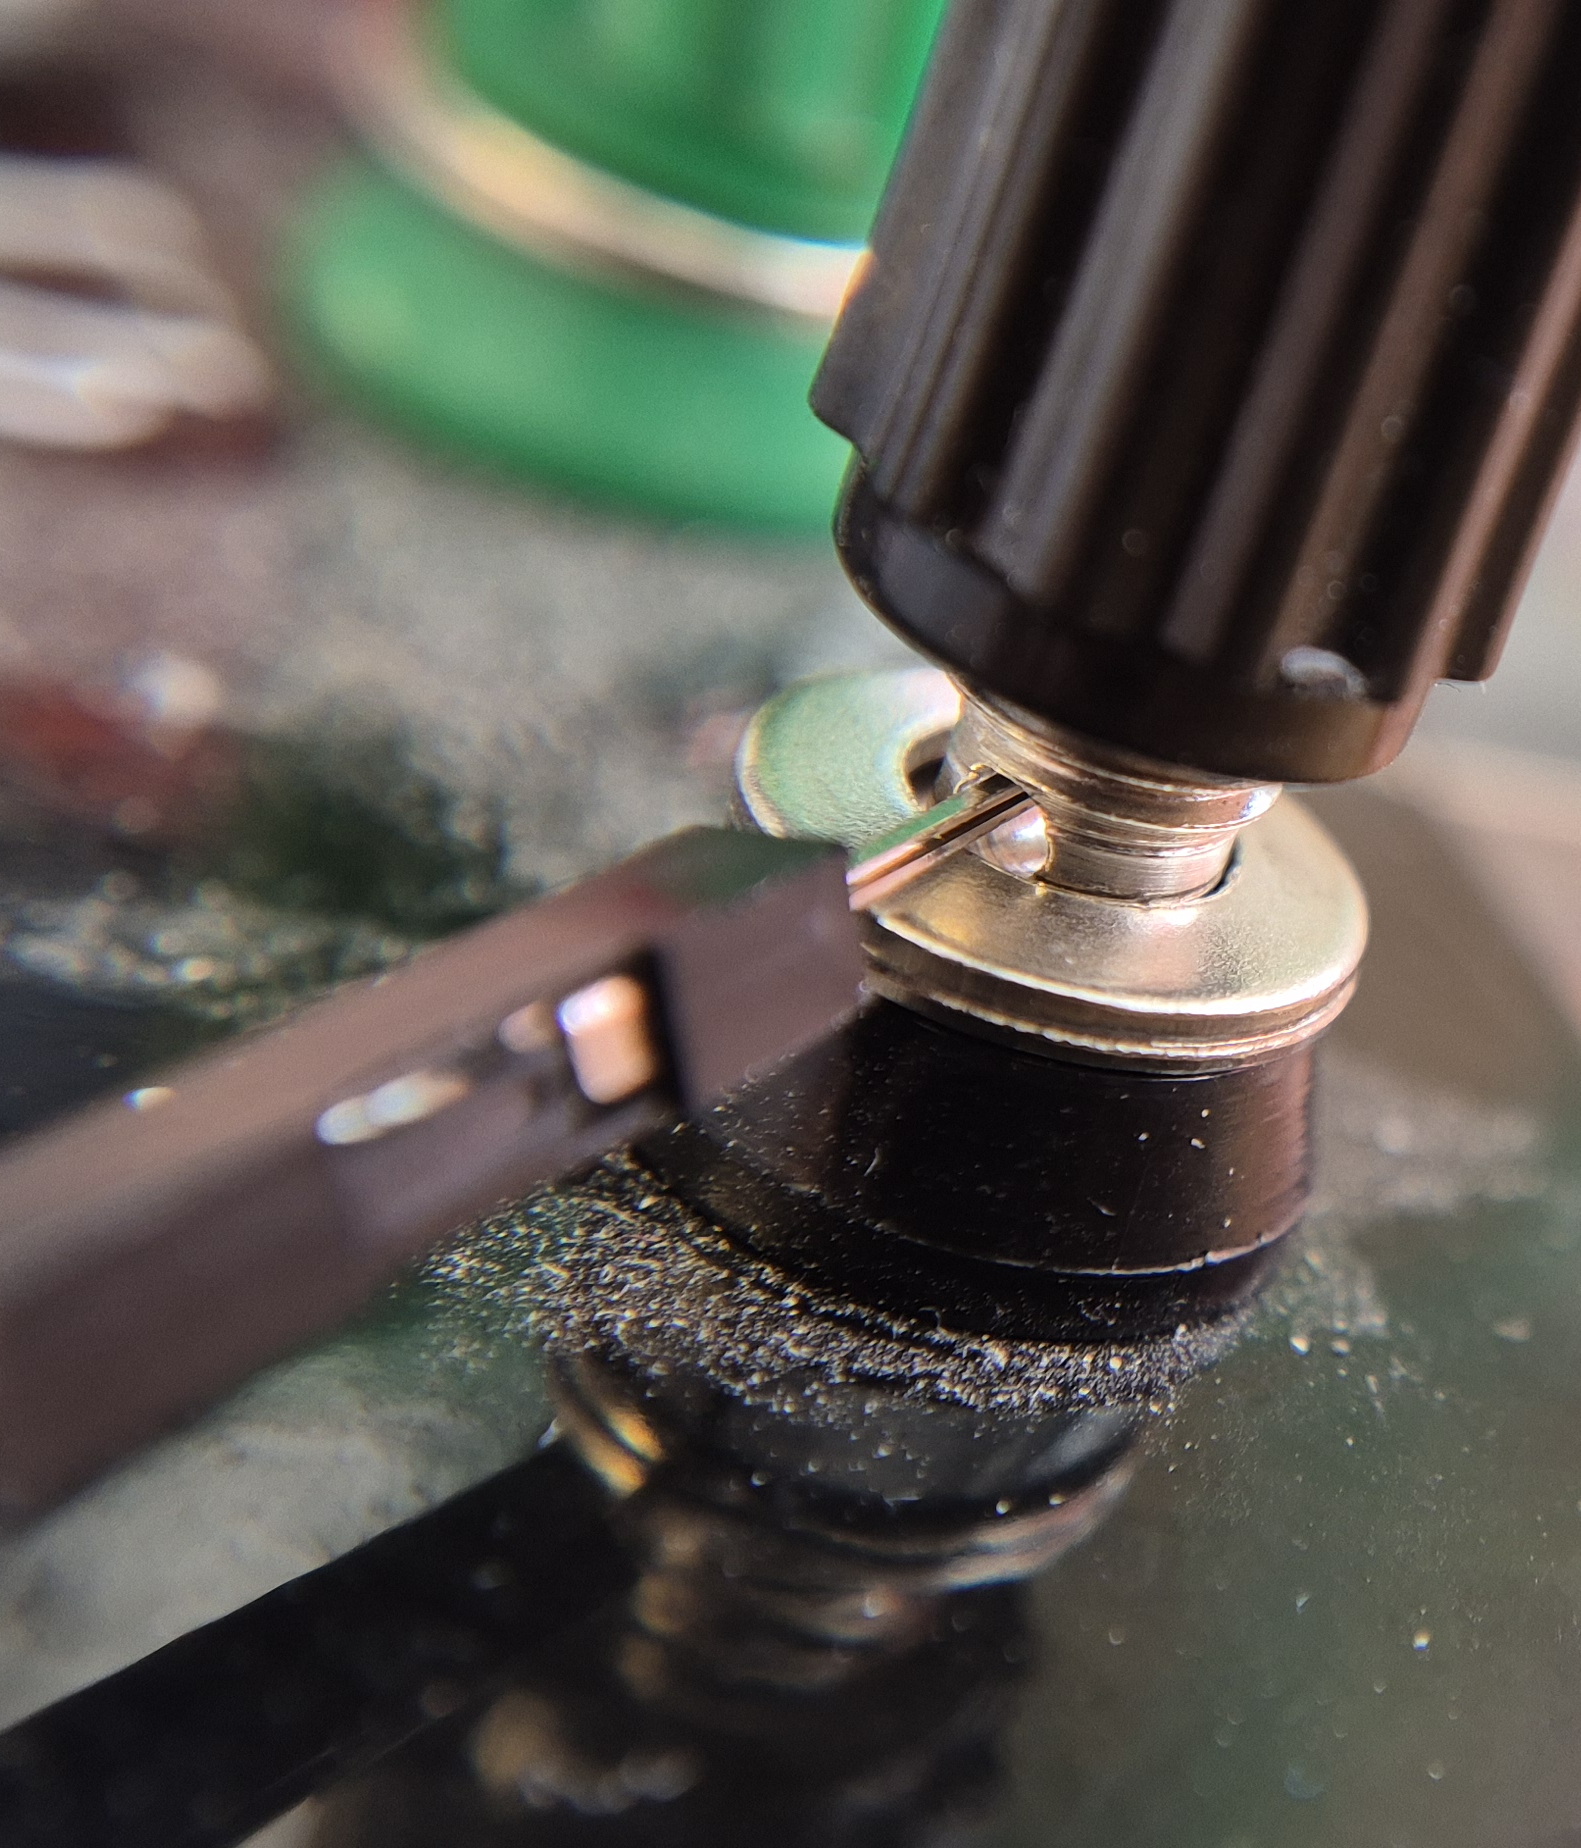
\includegraphics[height=\paperheight]{figures/breadboard_unscrewed.png}};
    \node[anchor=south east, outer sep=0pt] at (current page.south east)
      {\only<2->{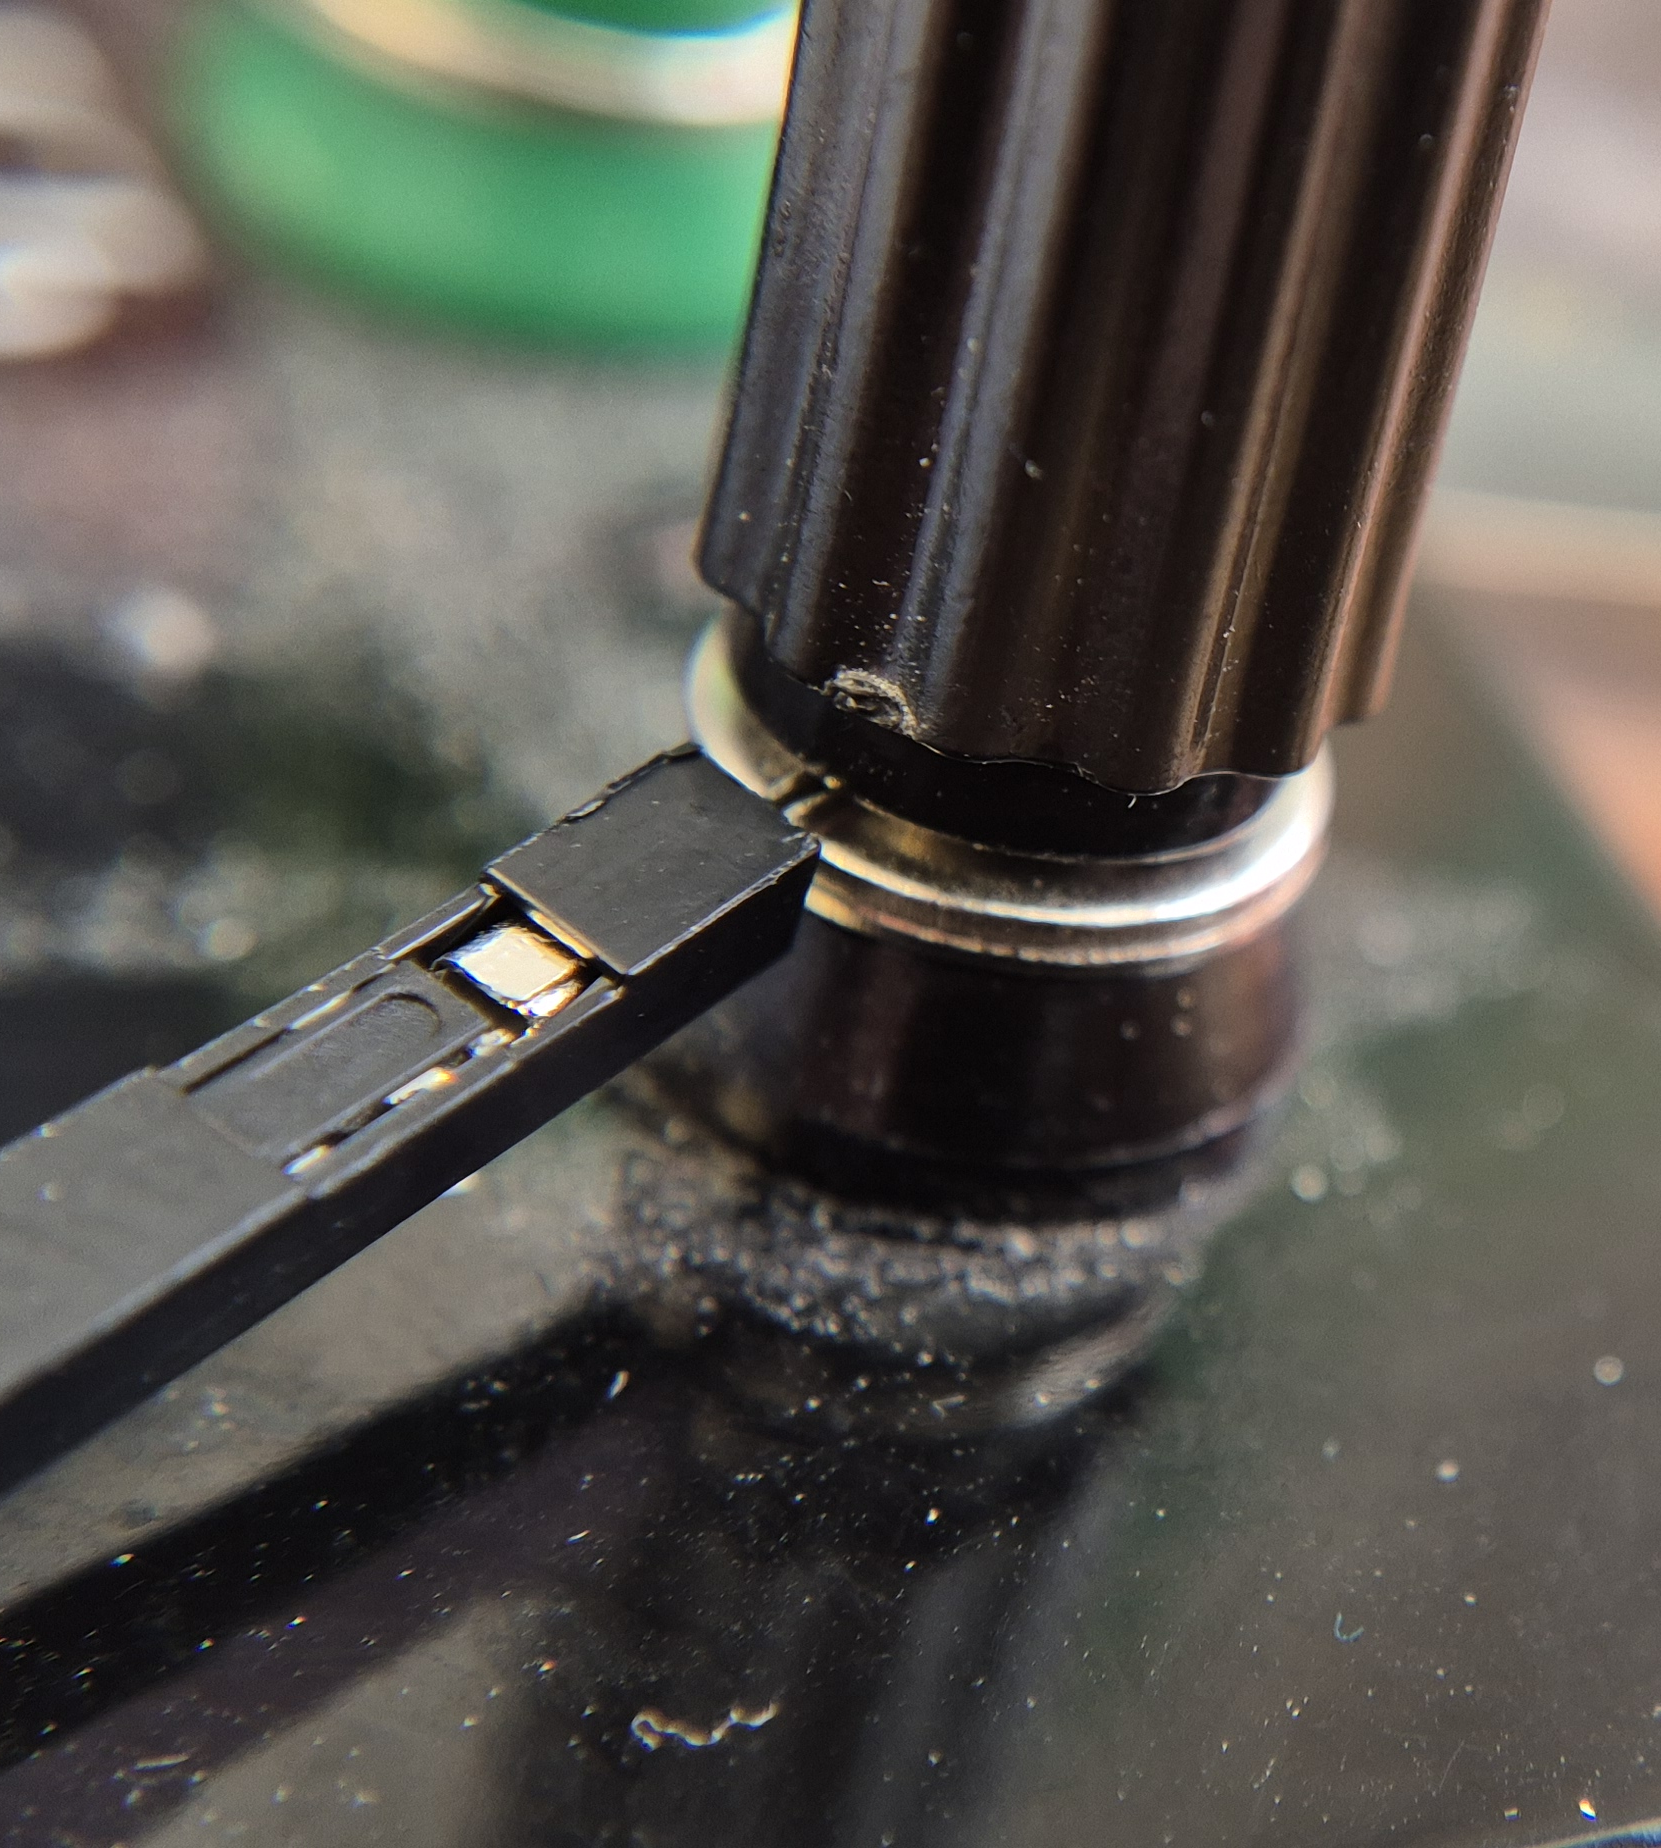
\includegraphics[height=\paperheight]{figures/breadboard_screwed.png}}};
    \node[
      anchor=north,
      outer sep=0pt,
      fill=black,
      fill opacity=0.65,
      text opacity=1,
      text=white,
      text width=0.88\paperwidth,
      align=center,
      inner xsep=0.25cm,
      inner ysep=0.18cm,
      font=\Large\bfseries
    ] at (current page.north) {Skruvterminal -- lossad till vänster, åtdragen till höger.};
  \end{tikzpicture}
\end{frame}

% bilden nedan kan göras bättre. Den kan fotograferas och klippas och göras till bilder med individuella steg.
\descriptionslide{figures/breadboard_bananas.png}{0.75}{Koppla jumpercables från skruvterminalerna\\ på breadboarden till respektive power rail.\\ Koppla banankablar från skruvterminalerna\\ på breadboarden till power supply.\\ Se till så powersupply-kanalen är avstängd!}{}

\mode<beamer>{
\sectionslide{Ställ på den inkopplade kanalen.\\[4mm] Lyser LEDen?\\ Mät spänningen över LEDen.}

\sectionslide{Mäta ström.}
} % end mode

\descriptionslide{figures/rigol-input-current.png}{0.5}{I detta läget \textit{kortsluter} multimetern --\\ alla kretsar måste \textit{brytas} för att kunna mätas.\\ Annars kortslutning och eldsvåda!}{}

\descriptionslide{figures/rigol_multimeter.png}{1}{}{
    \ringmarker{red}{0.76}{0.92}{0.45}
}
 
\descriptionslide{figures/fritzing.jpg}{1}{Koppla ur jumper wiren mellan power rail och LEDbenet (blå nedan). Röd multimeterprob mot LEDbenet och svart multimeterproben mot någon metallisk del av skruvterminalen. Mät strömmen som flyter genom LEDen.}{} 

\handoutnoteslide

\mode<beamer>{
% Analogt instrument - omkopplare för olika mätområden
\descriptionslide{figures/simpson_valjare.JPG}{0.9}{Börja alltid på största värdet!}{}
} % end mode

\frame{
    \frametitle{}
    \begin{tikzpicture}[remember picture,overlay]
        \node[at=(current page.center)] {
            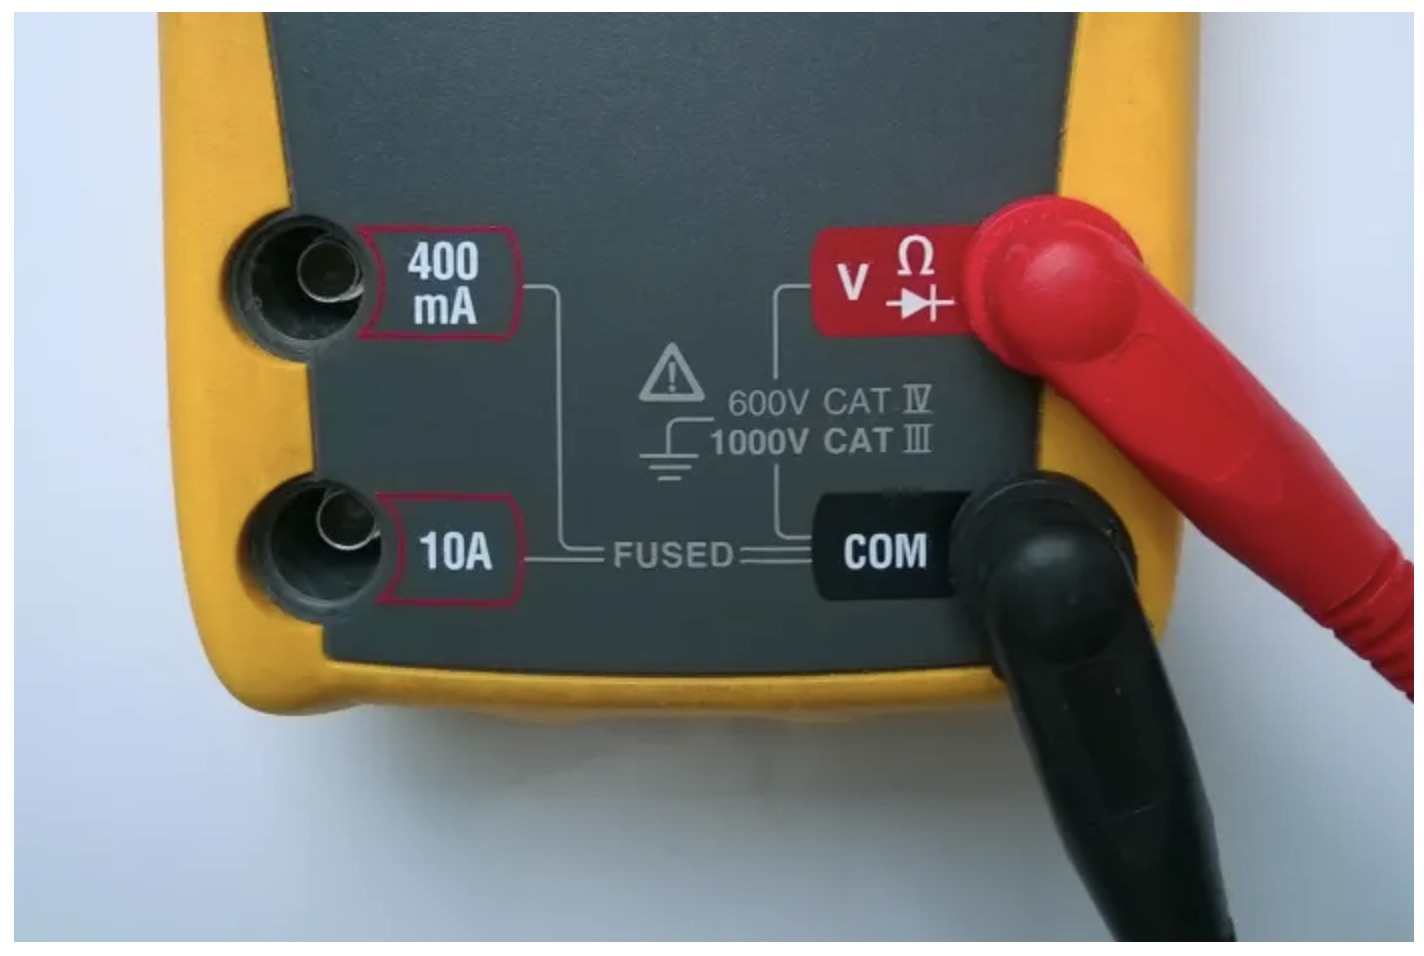
\includegraphics[keepaspectratio,
                                 width=\paperwidth,
                                 height=\paperheight]{figures/multimeter_probes_voltage.png}
            };
   			% Varför skall vi lära oss detta?
			\onslide<1->{
			\node[rotate=30, white] at (6,2){{\Huge Ganska säkert!}};
			}
    \end{tikzpicture}    
    }


\frame{
    \frametitle{}
    \begin{tikzpicture}[remember picture,overlay]
        \node[at=(current page.center)] {
            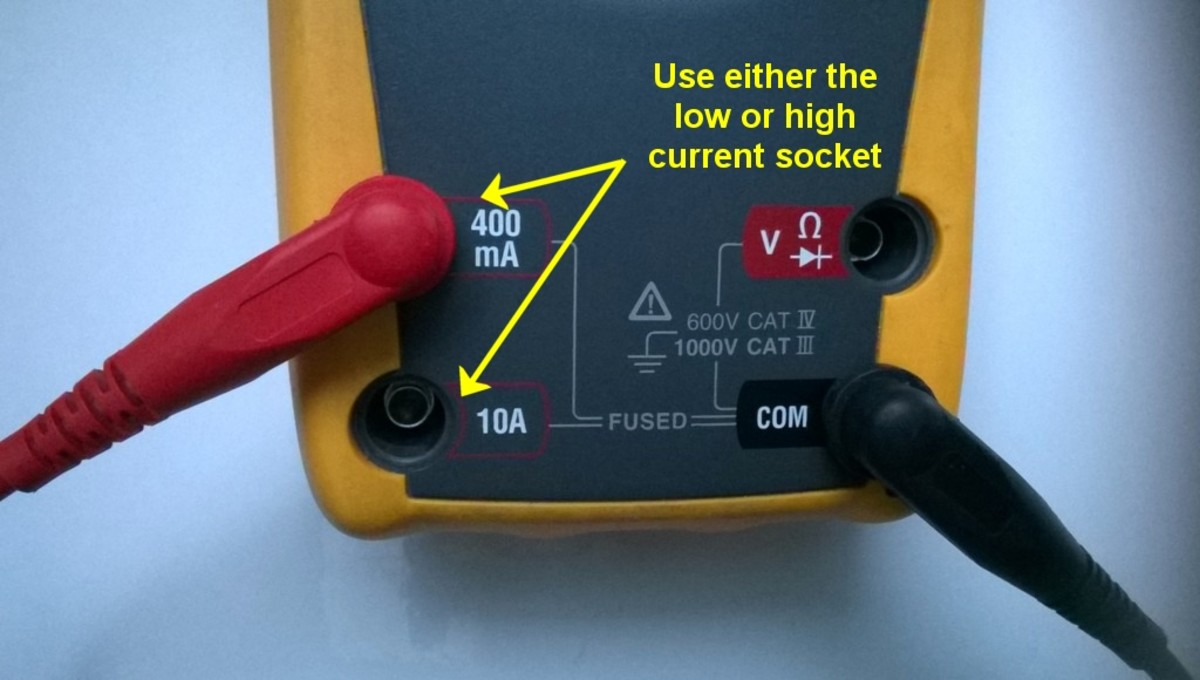
\includegraphics[keepaspectratio,
                                 width=\paperwidth,
                                 height=\paperheight]{figures/multimeter_probes_current.jpg}
            };
   			% Varför skall vi lära oss detta?
			\onslide<1->{
			\node[rotate=30, white] at (3,0.5){{\Huge  Osäkert! Varning!}};
			}
    \end{tikzpicture}    
    }


\frame{
\frametitle{Mäta spänning}
\resizebox{\textwidth}{!}{%
\begin{minipage}{.5\textwidth}
\centering
\begin{tikzpicture}[scale = 1, american]
    \draw (0, 0) 
    node[ground, rotate=-90] {}
    to[american voltage source=\qty{10}{\V}, invert, *-] (0, 2) 
    -- (2, 2) 
    to[R=\qty{470}{\ohm}, i=$I$] (2, 0)
	-- (0, 0)
    ;
    \draw (2, 2) 
    to[short,*-] (4, 2) 
    to[voltmeter] (4, 0) 
    to[short, -*] (2, 0)
    ;
\end{tikzpicture}\\
Spänning \alert{över} komponenter!
\end{minipage}}
}

\handoutnoteslide


\frame{
\frametitle{Mäta ström}
\resizebox{\textwidth}{!}{%
\begin{minipage}{.5\textwidth}
\centering
\begin{tikzpicture}[scale = 1, american]
    \draw (0, 0) 
    node[ground, rotate=-90] {}
    to[american voltage source=\qty{5}{\V}, invert, *-] (0, 2) 
    to[short, -*] (0.5, 2)
    to[ammeter,-*] (2.5, 2) 
    -- (3, 2)
    to[R=\qty{470}{\ohm}, i=$I$] (3, 0)
	-- (0, 0)
    ;
%    \draw (2, 2) 
%    to[short,*-] (4, 2) 
%    to[ammeter] (4, 0) 
%    to[short, -*] (2, 0)
%    ;
\end{tikzpicture}\\
Ström \alert{genom} komponenter!
\end{minipage}}
}

\handoutnoteslide


\frame{
\frametitle{Mäta motstånd}
\resizebox{\textwidth}{!}{%
\begin{minipage}{.5\textwidth}
\centering
\begin{tikzpicture}[scale = 1, american]
    \draw (2, 2) 
    to[R=\qty{470}{\ohm}] (2, 0)
    ;
    \draw (2, 2) 
    to[short, -*] (3, 2)
    -- (4,2)
    to[ohmmeter] (4, 0) 
    -- (3, 0)
    to[short, *-] (2, 0)
    ;
\end{tikzpicture}\\
Koppla loss komponenter för motståndsmätning!
\end{minipage}}
}

\handoutnoteslide


%%--------------------------------------------------
%% Ny frame
%%--------------------------------------------------
\begin{frame}[fragile]{Strömmar i kretsar}
  \begin{columns}
    \column{0.5\textwidth}
    \alert{Parallellkoppling:} Spänning samma över resistorer!\\
    Bestäm samtliga strömmar i kretsen.
    \onslide<2->{
      \[\frac{1}{R_{\mathrm{tot}}}=\frac{1}{R1}+\frac{1}{R2}+\ldots\]
    }
    \onslide<2->{
      \[ R_{\mathrm{tot}} = \left(\frac{1}{R1}+\frac{1}{R2}+\ldots\right)^{-1} \]
    }
    

    \column{0.5\textwidth}
    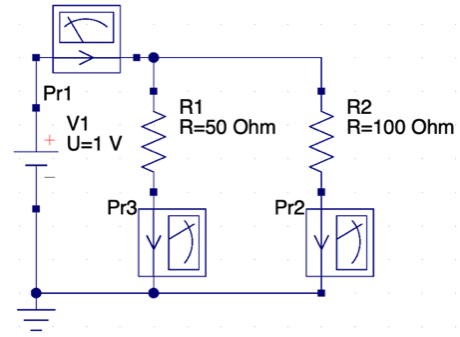
\includegraphics[width=\textwidth]{figures/parallellk.png}\\
  \end{columns}
\end{frame}


%%--------------------------------------------------
%% Ny frame
%%--------------------------------------------------
\begin{frame}[fragile]{Spänningar i kretsar}
  \begin{columns}
    \column{0.5\textwidth}
    \alert{Seriekoppling:} Strömmen samma genom resistorerna!\\
    Bestäm potentialen i $A$.
    \onslide<2->{
      \[R_{\mathrm{tot}}=R1+R2+\ldots\]
    }
    \column{0.5\textwidth}
    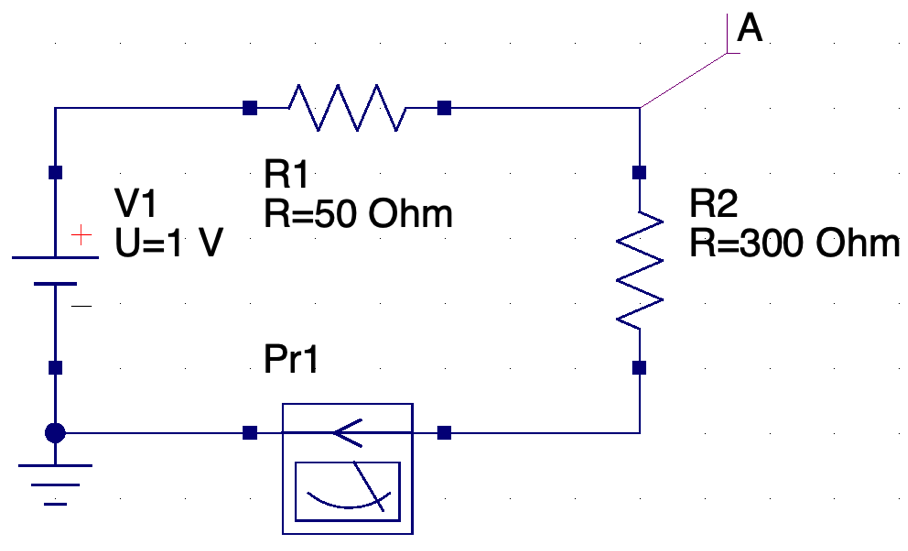
\includegraphics[width=\textwidth]{figures/seriek.png}\\
  \end{columns}
\end{frame}



%%--------------------------------------------------
%% Ny frame
%%--------------------------------------------------
 \begin{frame}\frametitle{Spänningsdelning, lägesgivare}
   \begin{columns}
   \centering
   \column{0.3\textwidth}
   \begin{circuitikz}[american] \draw
     node[ground]{}
     (0, 0)  to[battery2, invert, l_=V$_1$, *-] (0,4)
     (0, 4) -- (2, 4)
     to[R=R$_1$] (2, 2)
     to[R=R$_2$, v=$U_2$] (2, 0)
     (2,0) -- (0,0)    
 ;
 \end{circuitikz}
 \column{0.7\textwidth}
     \begin{itemize} % specificera label
       % beamer
     \item<2-> Spänningsdelning, strömmen $I=\frac{V_1}{R_1+R_2}$
       \item<3-> Spänning över $R_2$ blir då
         $U_2=R_2\frac{V_1}{R_1+R_2}$
         \onslide<4->{ \[U_2=V_1\frac{R_2}{R_1+R_2}\] }
         \item<5-> \emph{Spänningsdelningslagen}
 \end{itemize}
 \end{columns}
 \end{frame}
 \handoutnoteslide
 
%%--------------------------------------------------
%% Ny frame
%%--------------------------------------------------
\begin{frame}\frametitle{Spänningsdelning, lägesgivare -- exempel 2.5}
  \begin{columns}
  \centering
  \column{0.5\textwidth}
  \begin{circuitikz} \draw
    node[ground]{}
    (0, 0)  to[battery2, invert, l_=\qty{9}{V}, *-] (0,2)
    to[R=\qty{100}{\ohm}] (0, 4)
    (0, 4) -- (2, 4)
    to[R=\qty{200}{\ohm}, v=$U_{R200}$] (2, 2)
    to[R=\qty{300}{\ohm}] (2, 0)
    (2,0) -- (0,0)    
;
\end{circuitikz}
\column{0.5\textwidth}
Beräkna spänningen över \qty{200}{\ohm}-motståndet.\\
% \onslide<2-> {Spänningsdelningslagen ger:}
% \onslide<3-> {\[U_\mathrm{R200}=9\frac{200}{100+200+300}\mathrm{V}}\onslide<4->{=\qty{3}{\volt}\] }
\vspace{30mm}
\end{columns}
\end{frame}

\handoutnoteslide

\end{document}
